\chapter[The Periodic Flapping and Breathing of Saturn's Magnetodisc]{The Periodic `Flapping' and `Breathing' of Saturn's Magnetodisc}
\label{chap:equinox}

Periodic variations have been observed in many field and particle properties in Saturn's magnetosphere, modulated at a period close to the planetary rotation rate. Magnetic field observations by Cassini's magnetometer instrument suggest that in the outer magnetosphere (beyond ${\sim}$12 Saturn radii) Saturn's current sheet is periodically displaced with respect to the rotational equator, to a first approximation acting as a rotating, tilted disk. This manifests as a `flapping' mode when observed by the spacecraft. Recent studies suggest the magnetosphere also has a `breathing' mode, expanding and contracting with a period close to the planetary rotation rate. We model these two modes in tandem by combining a global, geometrical model of a tilted and rippled current sheet with a local, force-balance model of Saturn's magnetodisk, accounting for the magnetospheric size and hot plasma content. We simulate the breathing behavior by introducing an azimuthal dependence of the system size. We fit Cassini magnetometer data acquired on equatorial orbits from 23 Oct{\--}17 Dec 2009 (Revs 120{\--}122), close to Saturn equinox, in order that seasonal effects on the current sheet are minimized. We find that our model characterizes well the amplitude and phase of the oscillations in the data, for those passes that show clear periodic signatures in the field. In particular, the $B_\theta$ (meridional) component can only be characterized when the breathing mode is included. This study introduces calculations for an oscillating boundary, which provide a basis for understanding the complex relationship between current sheet dynamics and the periodic field perturbations.

\section{Introduction}\label{equinox:sec:intro}
Recent observations of Saturn's magnetic field suggest that the planetary dipole axis and rotation axis are aligned to $\leq\SI{0.06}{\degree}$ \citep{cao2011}. However despite this extremely high degree of axisymmetry, periodic variations have been observed in field and particle properties throughout Saturn's magnetosphere, modulated at a period close to the planetary rotation rate, summarized in \citet{carbary2013}. The location of the auroral oval \citep{provan2009b}, and the magnetopause \citep{clarke2010}; the magnetic field \citep{espinosa2000, andrews2008}; electron densities \citep{morooka2009}; ions \citep{burch2009, nemeth2011, szego2011}; and energetic neutral atoms \citep{paranicas2005}, all show some relationship with an effective Saturn longitude. Therefore creating a reliable Saturn longitude system for organizing such observations has been a key focus in the scientific community.

Initially, periodicities in radio observations of Saturn's auroral regions from the \textit{Voyager} spacecraft suggested a planetary rotation rate of $\SI{10.657}{\hour}$, and this was used to create an initial Saturnian longitude system \citep{desch1981}. However data from the \textit{Ulysses} and \textit{Cassini} missions then revealed that this radio period actually drifted over time, and therefore could not be directly associated with a source in Saturn's deep interior \citep[e.g.][]{gurnett2005}. A reanalysis of magnetometer data from the \textit{Voyager} and \textit{Pioneer} missions showed a similar periodic behavior in the magnetic field, leading to the development of a `camshaft' model of a rotating magnetic anomaly causing the perturbations \citep{espinosa2003b}. To further complicate the picture, two distinct periods were then discovered by Cassini in the radio signal (Saturn Kilometric Radiation, or SKR), associated separately with the Northern and Southern hemispheres \citep{gurnett2009}. This phenomenon is also observed in more recent \textit{Cassini} magnetic field observations \citep[e.g.][]{andrews2010,provan2012}. In these and other studies, such as \citet{hunt2014}, a picture has been developed of how these magnetic perturbations are generated, by dual large-scale field-aligned current systems that rotate at slightly different rates. The magnetic signatures of each current system are dominant in the respective Northern and Southern hemispheres. The physical origins of these current systems are still not fully understood, but are thought to be associated with twin atmospheric vortices flowing in the polar upper atmosphere and ionosphere in each hemisphere \citep{jiaandkivelson2012, smith2012, southwood2014, smith2016}. During the initial \textit{Cassini} mission, the southern magnetic perturbation was dominant over the northern, and had a longer period of ${\sim}\SI{10.8}{\hour}$ compared to ${\sim}\SI{10.6}{\hour}$. However after Saturn equinox in August 2009, the two perturbations slowly converged in terms of both time period and amplitude, before diverging again \citep{andrews2012}.

In this study we focus on the effect of these dual rotating magnetic perturbations on Saturn's outer magnetosphere. To do this, it is helpful to first consider the picture put forth in \citet{andrews2010, provan2011} and references therein, of the two hemispheric perturbations being approximated by rotating transverse dipoles, each with associated magnetic field only felt in the respective hemisphere. In the magnetosphere's equatorial `core' region, within radial distances of ${\sim}10{\--}\SI{15}{R_S}$ (where $\si{R_S}$ is Saturn's radius, $\SI{60268}{\km}$) and thus within the magnetic shells of the associated field-aligned currents \citep[e.g.][]{southwood2007}, the resulting magnetic perturbation field is rotating and quasi-uniform in magnitude. On higher-latitude field lines, and beyond the core region, the perturbation field can be approximated in each hemisphere by a dipole magnetic field whose axis lies in the rotational equatorial plane. The influence of these magnetic perturbations on the global magnetodisk structure is shown by the diagram in Figure~\ref{equinox:fig:CowleyTDdiagrams}, reproduced from \citet{cowley2017a}. The magnetospheric magnetic field, made up of Saturn's planetary dipole field and the magnetodisk field, is shown by the black lines in panels (a) and (c), whilst the perturbation fields associated with the Northern and Southern hemispheres are shown in blue and red respectively. The effect of these perturbation fields on the total magnetospheric magnetic field is then shown by the black lines in panels (b) and (d). The direction in which the effective `transverse dipole' points can be ascertained via an analysis of the oscillations in the magnetic field data \citep[e.g.][]{provan2009}, defined in each hemisphere by a phase $\Psi_\mathrm{N,S} = \SI{0}{\degree}$ and thus used to define a physically meaningful longitude system for the planet.
\begin{figure}
\centering
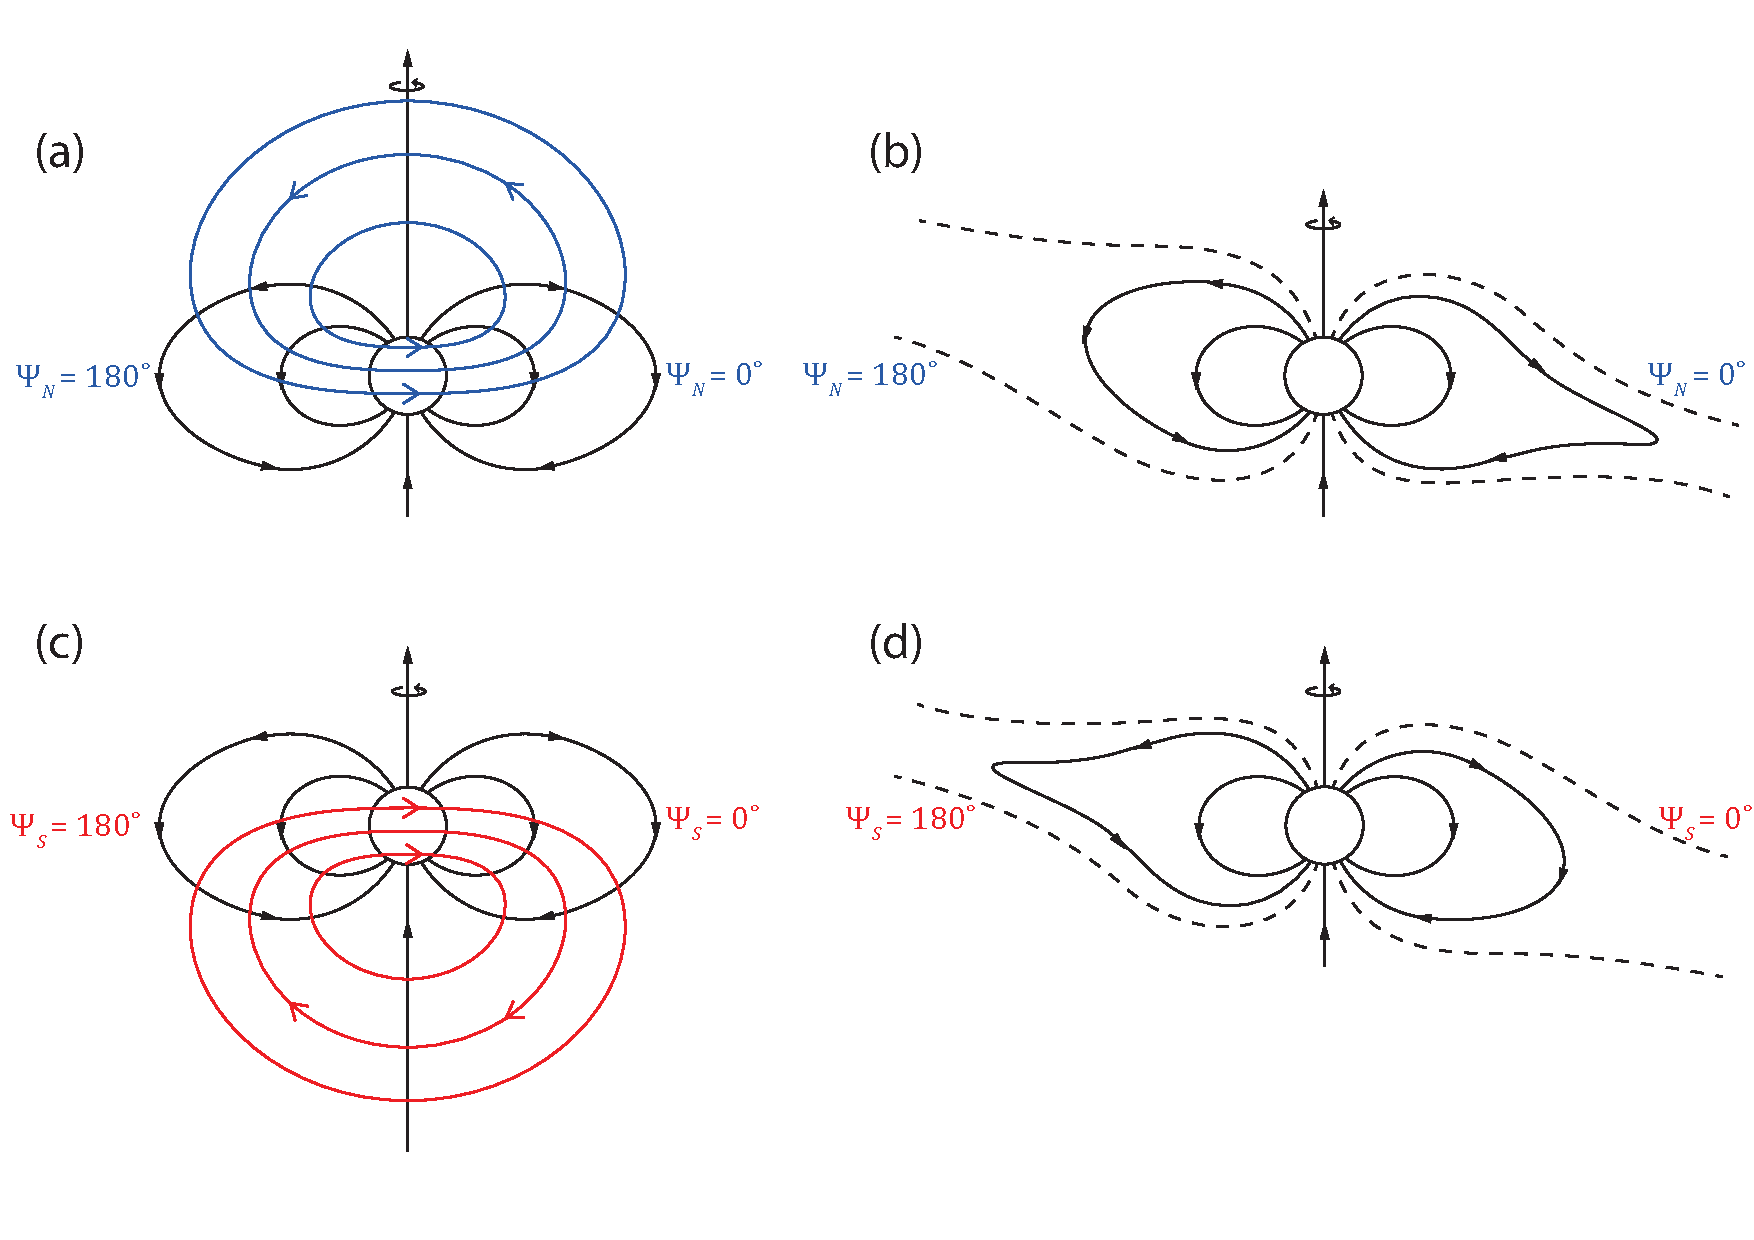
\includegraphics[width=0.7\textwidth]{equinox/CowleyTDdiagrams.pdf}
\caption[Sketches of hemispheric rotating magnetic perturbation fields, from \citet{cowley2017a}.]{Sketches showing the planetary magnetodisk magnetic field in black lines, and the magnetic field associated with the northern and southern hemispheric magnetic perturbations, in blue and red respectively. Panels (b) and (d) show the result of the superposition of the magnetodisk and perturbation magnetic fields shown in (a) and (c). Reproduced from \citet{cowley2017a}.}
\label{equinox:fig:CowleyTDdiagrams}
\end{figure}

A key effect of these magnetic perturbations on Saturn's magnetodisk is a periodic motion of the equatorial current sheet above and below the rotational equator, or `flapping' behavior as perceived by a stationary observer. This is a separate phenomenon to the displacement of the entire current sheet northwards into a bowl-like shape observed by \citet{arridge2008warp} during the initial \textit{Cassini} mission, which was due to the incoming direction of the solar wind plasma impacting the magnetopause from the south during Saturn's southern summer. In the transverse dipole approximation, this flapping we describe can be understood as follows. At $\Psi_\mathrm{N,S} = \SI{0}{\degree}$, the radial component of the perturbation field adds to the planetary magnetodisk field north of the equator, and subtracts from the background field south of the equator. The opposite is true at $\Psi_\mathrm{N,S} = \SI{180}{\degree}$. Magnetic pressure balance must be approximately maintained across the lobes of (regions just outside) the current sheet and thus this has the net effect of a rotating perturbation, acting to displace the equatorial current sheet southward below the rotational equator at the particular longitude defined by $\Psi_\mathrm{N,S} = \SI{0}{\degree}$, and northward at the diametrically opposite longitude, as shown in Figure~\ref{equinox:fig:CowleyTDdiagrams} b, d. As the whole pattern rotates, this rotating tilted magnetodisk appears to a stationary observer as a periodic vertical flapping of the current sheet, as it passes above and then below the rotational equator once per rotation period. 

This behavior has been detected, and quantified to some extent, in studies using various \textit{Cassini} datasets. In \citet{southwood2007}, the authors analyzed signatures of periodic equatorial current sheet crossings observed in the magnetic field data measured by \textit{Cassini's} magnetometer (MAG) instrument \citep{dougherty2004} on equatorial orbits in 2006. They determined that, in the outer magnetosphere beyond ${\sim}12{\--}\SI{15}{R_S}$, the total magnetic field can be approximated by a rotating tilted disk, with a tilt angle of ${\sim}12{\--}\SI{15}{\degree}$ relative to the spin axis. This is in broad agreement with a study by \citet{arridge2011}, who fitted a model of a tilted and rippled current sheet to MAG and plasma data measured by \textit{Cassini's} CAPS/ELS instrument (\textit{CAssini} Plasma Spectrometer/ELectron Spectrometer) \citep{young2004} to orbits from 2006. They found that a value of $\SI{12}{\degree}$ for the effective current sheet tilt provided a good agreement between their model and the data, and that smaller values could not reproduce the amplitudes of the oscillations in the data. In contrast, in \citet{provan2009} the authors analyzed magnetic field data from subsequent higher-latitude \textit{Cassini} orbits and found smaller values for an effective dipole tilt of ${\sim}5{\--}\SI{10}{\degree}$, and that the best fit value depended on the component of the magnetic field vector being analyzed. 

As pointed out in \citet{provan2009}, this kind of analysis does not establish the influence of the relative phases of the southern and northern perturbations on the current sheet flapping. The studies discussed so far are based on \textit{Cassini} observations made when the southern perturbation was dominant in amplitude, and thus the observed current sheet tilt was associated with this perturbation only. However, as previously mentioned, after Saturn equinox the two perturbations became similar in amplitude, and so it is important to consider the effect of both. Figure~\ref{equinox:fig:CowleyTDdiagrams} illustrates that a maximum current sheet displacement would be observed when the two perturbations are in phase, such that the meridians defined by $\Psi_\mathrm{N} = \SI{0}{\degree}$ and $\Psi_\mathrm{S} = \SI{0}{\degree}$ spatially coincide, and a minimum displacement arises when these meridians are diametrically opposite, and the perturbations are in antiphase. Indeed \citet{provan2012} observed in the magnetic field data that the current sheet oscillation was a maximum when the two perturbations were in phase, and some modeling studies such as \citet{jiaandkivelson2012} and \citet{cowley2017a} have also investigated this kind of behavior. However there is still much to be understood, particularly for intermediate perturbation phase differences, and the effect of the change of phase with radial distance in the outer magnetosphere. In this study we look at these effects in more detail.

The other important effect of these magnetic perturbations is the current sheet `breathing' behavior. That is, a compressional disturbance in the magnetodisk. While the rotational disturbance that causes the flapping behavior is mainly associated with the \textit{radial} component of the perturbation magnetic field, the compressional disturbance is mainly associated with the \textit{meridional} component. Again looking at Figure~\ref{equinox:fig:CowleyTDdiagrams}, we can see that for the northern perturbation, the meridional component subtracts from the planetary magnetodisk field at $\Psi_\mathrm{N} = \SI{0}{\degree}$, and adds at $\Psi_\mathrm{N} = \SI{180}{\degree}$. In contrast for the southern perturbation, the meridional component adds to the planetary magnetodisk field at $\Psi_\mathrm{S} = \SI{0}{\degree}$, and subtracts at $\Psi_\mathrm{S} = \SI{180}{\degree}$. Where the perturbation field enhances the planetary magnetic field, this causes a compression of the magnetic field lines into a more dipolar configuration, associated with a thickening of the equatorial current sheet, observed by a stationary observer as a `breathing in'. At the opposite longitude, the reduction in the meridional component of the magnetodisk magnetic field causes an extension of the magnetic field lines into a more disk-like configuration, associated with a thinner and more extended current sheet. Unlike the case of the flapping perturbation, this breathing perturbation occurs at opposite phase longitudes for each hemisphere, and so we would expect to observe a maximum compressional disturbance when the northern and southern perturbations are $\SI{180}{\degree}$ out of phase.

This behavior was also observed in \citet{provan2012}, who found that the thickness of the current sheet was modulated by a factor of ${\sim}2$ when the magnetic perturbations were in antiphase. More recently, \citet{thomsen2017} looked in detail at the expected magnetic field signatures for intermediate perturbation field phase relationships, as a companion study to \citet{cowley2017a}. These studies found instances of `sawtooth' shaped signatures in the magnetic field data during current sheet crossings, and, through a comparison with various modeling results, suggested that this was associated with a periodic thickening and thinning of the magnetospheric current sheet. A further study by \citet{cowley2017b} suggests a complex relationship between current sheet thickness in each hemisphere and intermediate perturbation phase differences. In MHD modeling studies there is also evidence for this periodic breathing behavior in the middle magnetosphere \citep{ramer2016}, and a periodic perturbation in the magnetopause boundary location \citep{kivelson2014}, which may be related. As previously mentioned, \citet{clarke2010} also found evidence using \textit{Cassini} magnetometer data that the magnetopause boundary moves periodically by up to $\SI{5}{R_S}$ in the post-noon local time sector.

In this study we attempt to draw these various strands together, and investigate both the flapping and breathing behavior of Saturn's magnetodisk. We use a local, force-balance magnetic field and plasma model of Saturn's magnetodisk adapted from \citet{achilleos2010a}, and anchor it to a global, geometric model of the current sheet location adapted from \citet{arridge2011} in order to model a magnetodisk that displays both behaviors. We compare our model magnetic field predictions to measurements made by \textit{Cassini's} magnetometer on three equatorial orbits made shortly after Saturn equinox in August 2009, in order that the aforementioned seasonal effect on the current sheet shown by \citet{arridge2008warp} is minimized. We fit parameters that describe the tilt of the current sheet, and the longitudes of the maximum rotational (flapping) and compressional (breathing) disturbances, for each \textit{Cassini} pass in order to quantitatively understand how the relative phase of the hemispheric magnetic perturbations affects the magnetodisk structure. In Section \ref{equinox:sec:method} we discuss how the tilted, rippled current sheet model from \cite{arridge2011} simulates the flapping of the current sheet. We also describe the basis of the \citet{achilleos2010a} model, how we choose appropriate model parameters for our data set, and the modifications we make to it in this study. We also explain how we simulate breathing behavior by varying the magnetodisk model radius we use as a function of longitude. In Section~\ref{equinox:sec:results} we discuss the best fit parameters we find for each \textit{Cassini} pass in our data set, and what they indicate regarding the variability of the flapping and breathing behavior. We conclude with a summary and discussion of potential future work in Section~\ref{equinox:sec:conclusions}.

\section{Method}\label{equinox:sec:method}
\subsection{Data}
In this study we analyze \textit{Cassini} magnetometer data acquired on three equatorial orbits from 23 October{\--}17 December 2009 (Revs 120{\--}122), closely following Saturn equinox in August 2009. This interval is chosen in order that the seasonal effect of the current sheet deformation into a `bowl' shape \citep[e.g.][]{arridge2008warp} is minimized, and the current sheet is crossed numerous times. We only analyze data observed beyond \SI{12}{R_S} in cylindrical radial distance relative to the rotation / dipole axis, where we expect this dynamical behavior of the current sheet to occur. The choice of \SI{12}{R_S} in particular is discussed in detail in the next section. The data set is further restricted to ensure all observations are made within the magnetosphere proper by comparing with the list of magnetopause crossings made by \textit{Cassini} provided in the study by \citet{pilkington2015}, and comparing local MAG and CAPS-ELS observations to signatures described in that study, to determine whether \textit{Cassini} was inside or outside the magnetosphere at a given time. We further excluded data within 6 hours of a magnetopause crossing.

These trajectories are shown by the red-blue path in Figure~\ref{equinox:fig:cassinitrajectory}, with Saturn shown by the solid circle at the origin. The KSMAG coordinate system used represents a rotation about the $y$ axis of the more standard KSM coordinate system. In KSMAG, the $z$ axis points along Saturn's rotation/dipole axis, the $x$ axis is oriented such that the $x-z$ plane contains the planet-Sun direction, and the $y$ axis completes the right-handed set. A typical model magnetopause surface from \citep{pilkington2015} is shown by the black dashed line. In this data set the maximum radial distance of \textit{Cassini} from the planet is ${\sim}\SI{42.4}{R_S}$, the maximum distance of \textit{Cassini} above/below the rotational equator is $z_\mathrm{KSMAG}\approx +0.3/\SI{-1.2}{R_S}$, and the range in magnetic local time is ${\sim}$15:45 to 22:45. Since the spacecraft flies close to the rotational equator throughout this interval, we would expect to see near-symmetric oscillations in the radial component of the magnetic field, if the mean position of the current sheet also lies close to the rotational equator.
\begin{figure}
\centering
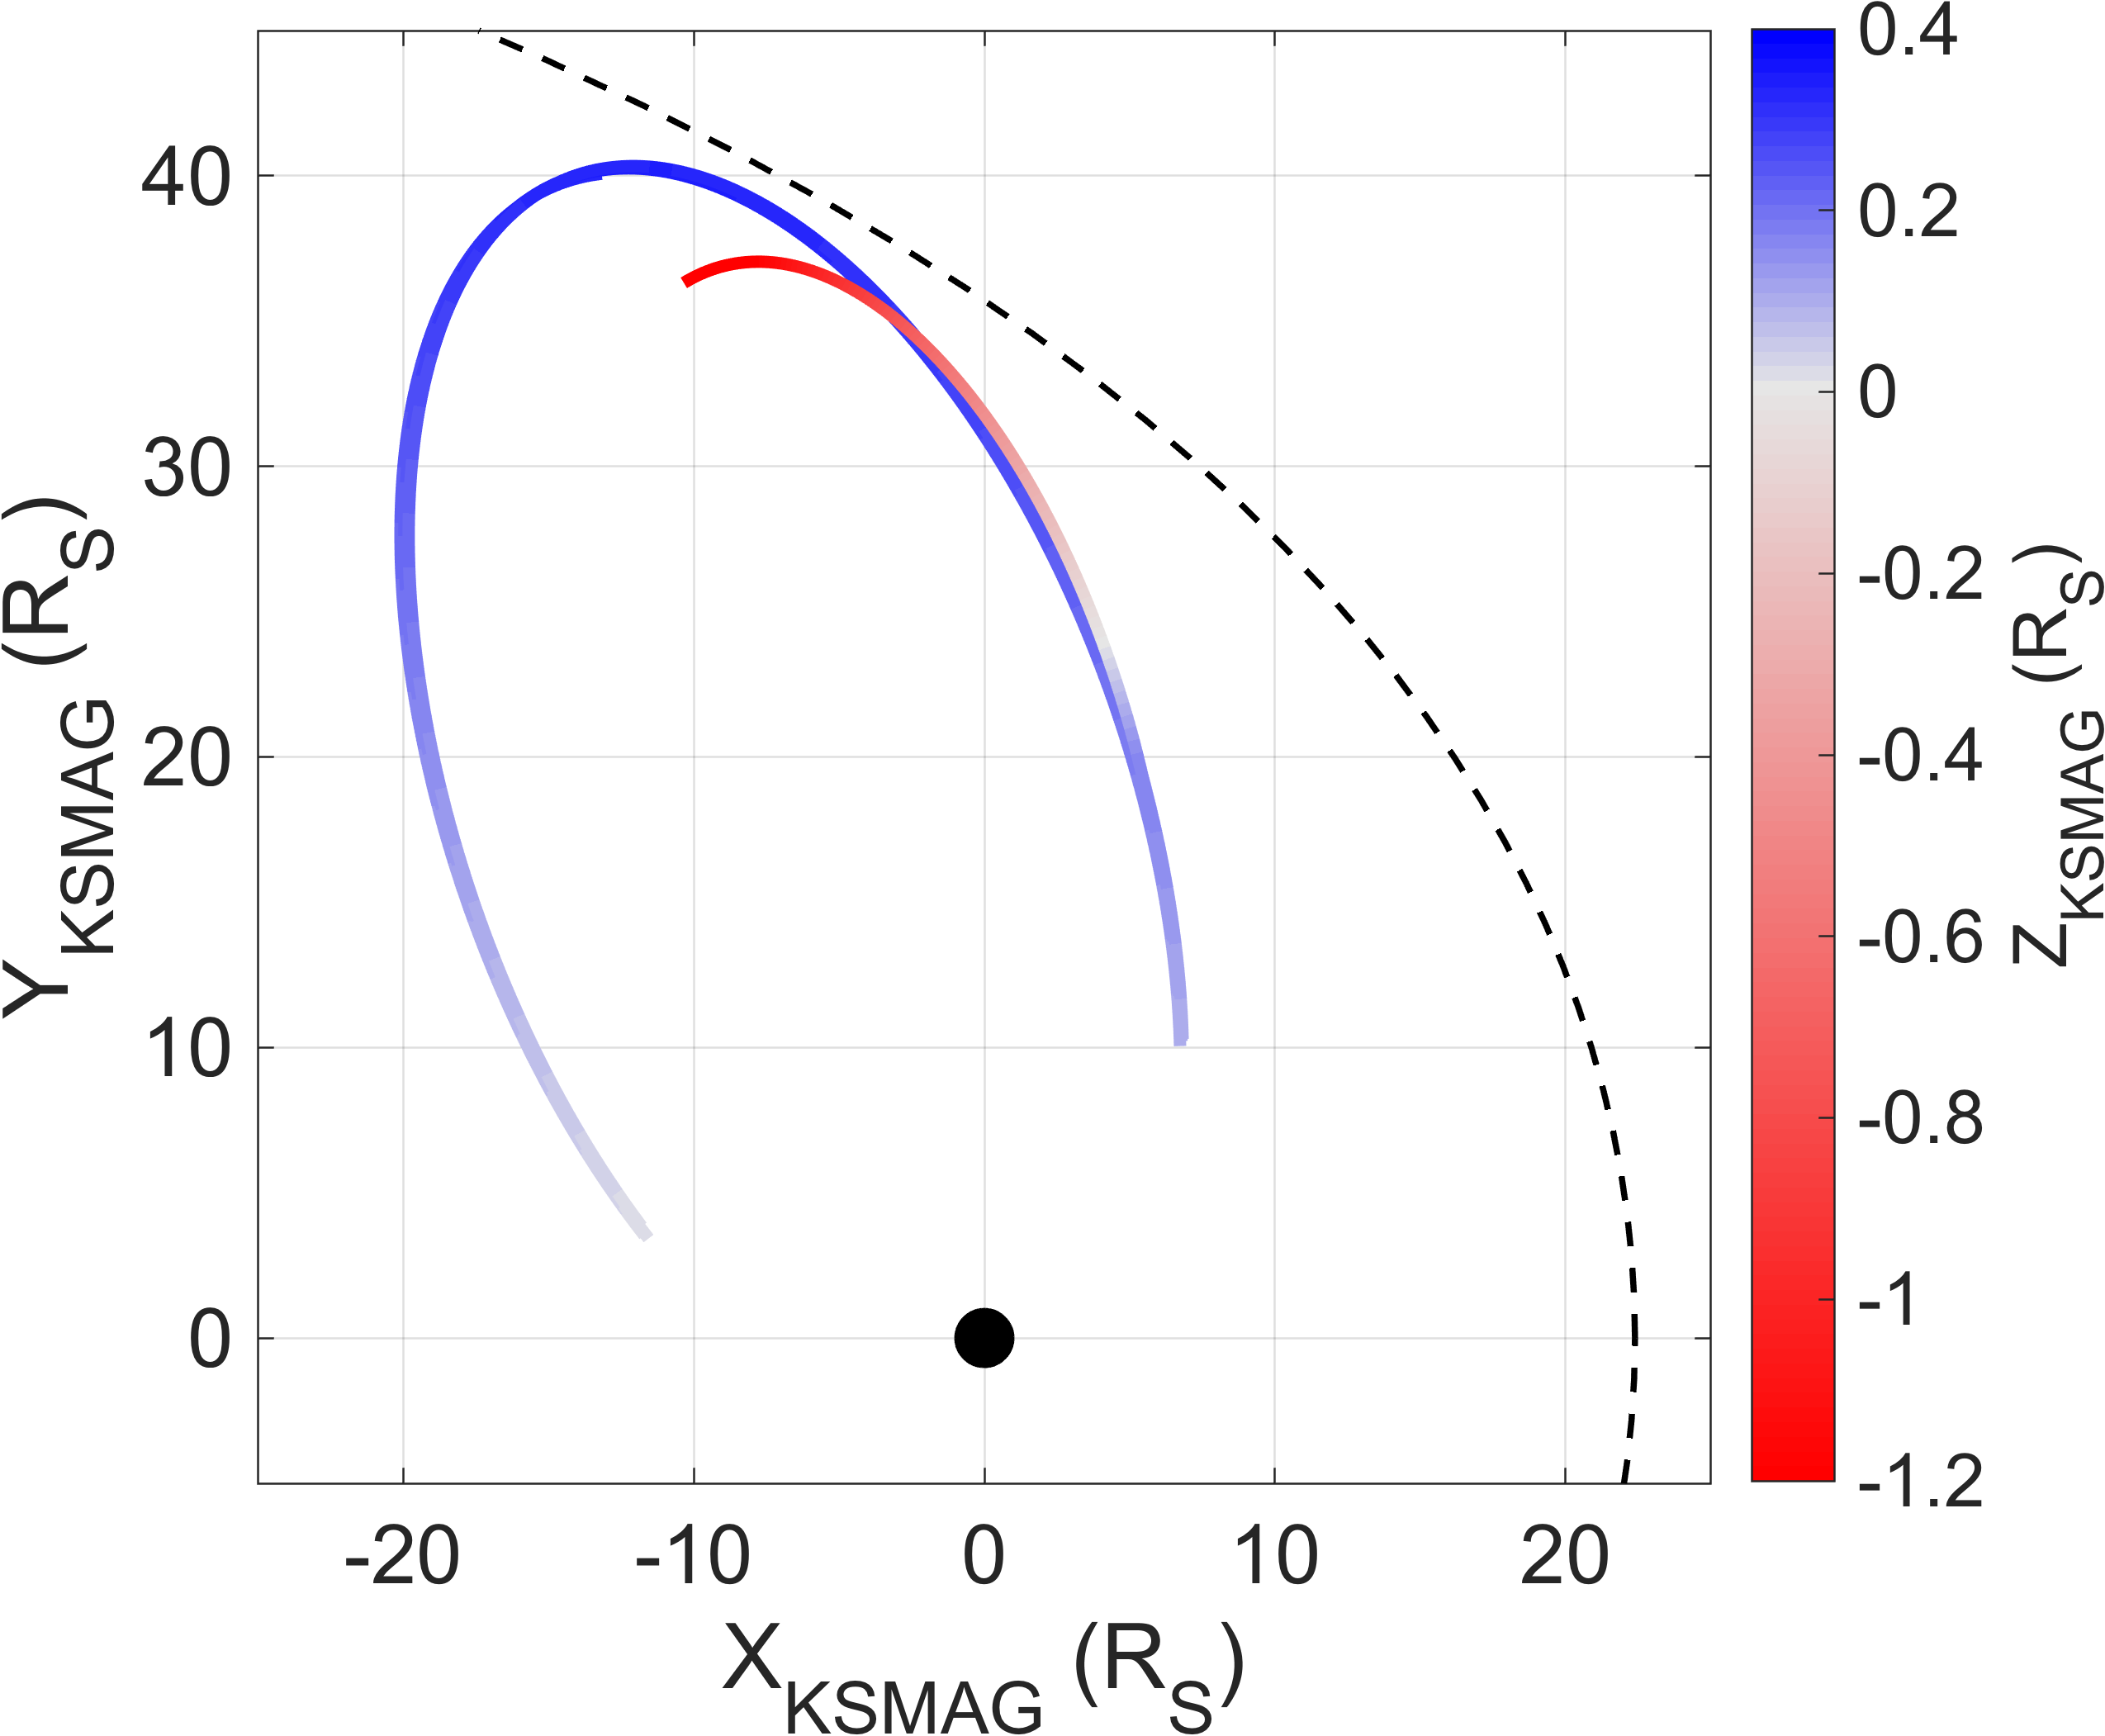
\includegraphics[width=0.6\textwidth]{equinox/cassinitrajectory.png}
% when using dvips, use .eps file:
% \includegraphics[width=20pc]{figsamp.eps}
\caption[\textit{Cassini} spacecraft trajectory for 23 October – 17 December 2009.]{The \textit{Cassini} spacecraft trajectory for the period 23 October{\--}17 December 2009 (Revs 120{\--}122), with an anticlockwise orbit. Colorbar shows height above and below Saturn's rotational/dipole equator. A typical model magnetopause surface from \citet{pilkington2015} is shown by the black dashed line.}
\label{equinox:fig:cassinitrajectory}
\end{figure}

\subsection{Current Sheet Surface Model}\label{equinox:sec:cssmodel}
To model the changing location of Saturn's equatorial current sheet over time, we use a structural model first applied to Saturn by \citet{arridge2011}, simplified to exclude the aforementioned bowl-like deformation associated with solstice conditions. The approach in that study was itself a continuation of analogous studies of Jupiter's magnetodisk \citep[e.g.][]{kivelson1978,khurana2005}. The model describes a current sheet effectively tilted from the rotational equator by an angle $\theta_\mathrm{T}$ beyond a cylindrical radial distance $\rho_0$, such that the height of the current sheet above the rotational equator $z_\mathrm{CS}$ is described by
\begin{equation}\label{equinox:eq:zcs}
z_\mathrm{CS} = \tan(\theta_\mathrm{T})(\rho-\rho_0)\cos(\lambda-\lambda_0)
\end{equation}
for $\rho > \rho_0$, where $\rho_0$ is a scale length in cylindrical radial distance which controls the amplitude of the perturbation. We use $\rho_0 = \SI{12}{R_S}$ in this study, in line with previous results from \citet{southwood2007} and \citet{arridge2011}, which suggested that this type of behavior only becomes significant beyond the magnetic shells of field-aligned currents, as discussed in Section~\ref{equinox:sec:intro}. $\lambda$ is an effective phase of this rotating perturbation, related to Saturn longitude $\lambda_\mathrm{MS}$ by
\begin{equation}\label{equinox:eq:lambda}
\lambda = \lambda_\mathrm{MS} - (\rho-\rho_0)\Omega_\mathrm{S}/v_\mathrm{W},
\end{equation}
such that the tilted current sheet pattern rotates at a rate close to the planetary rotation rate. For $\lambda_\mathrm{MS}$ we use the magnetic longitude system of \citet{andrews2012}, based on the magnetic field perturbation signal observed specifically in the Southern hemisphere, ($\Psi_\mathrm{S}$ in Figure~\ref{equinox:fig:CowleyTDdiagrams}), as this signal was at a similar or greater amplitude than the northern magnetic field perturbation signal for the period studied here \citep{andrews2012}. However we do consider the phase difference between the northern and southern signals when interpreting our results, later in this study. $\lambda_0$ is an offset parameter which describes the `phase front' of the maximum vertical displacement of the current sheet from the rotational equator relative to $\lambda$, which is equivalent to the magnetospheric longitude $\lambda_\mathrm{MS}$ at the distance $\rho = \rho_0$. $\lambda_0$ is thus effectively a `prime meridian' for this perturbation. The second term in equation~\ref{equinox:eq:lambda} introduces a radial delay in this perturbation, to account for the time taken for the magnetic perturbation to propagate radially outwards from its source, at an effective wavespeed $v_\mathrm{W}$. This causes a spiral-like pattern in the elevation of the current sheet surface. $\Omega_\mathrm{S}$ is a variable angular velocity close to the planetary rotation rate, corresponding to the angular velocity of the rotating perturbation defined by the $\lambda_\mathrm{MS}$ longitude system used here. These two terms can be represented by the single delay parameter
\begin{equation}\label{equinox:eq:D}
D = \Omega_\mathrm{S}/v_\mathrm{W},
\end{equation}
where $D$ has units of $\si{\degree/R_S}$. The corresponding spiral pattern in the current sheet structure can be seen in Figure~\ref{equinox:fig:cssurfacemodel}, which shows an example model current sheet surface with typical $D$, $\theta_\mathrm{T}$ and $\rho_0$ parameters as described in the caption. Also shown is a curve of constant phase passing through the maximum $z_\mathrm{CS}$ at each radial distance, corresponding to $\lambda=\lambda_0$.
\begin{figure}
\centering
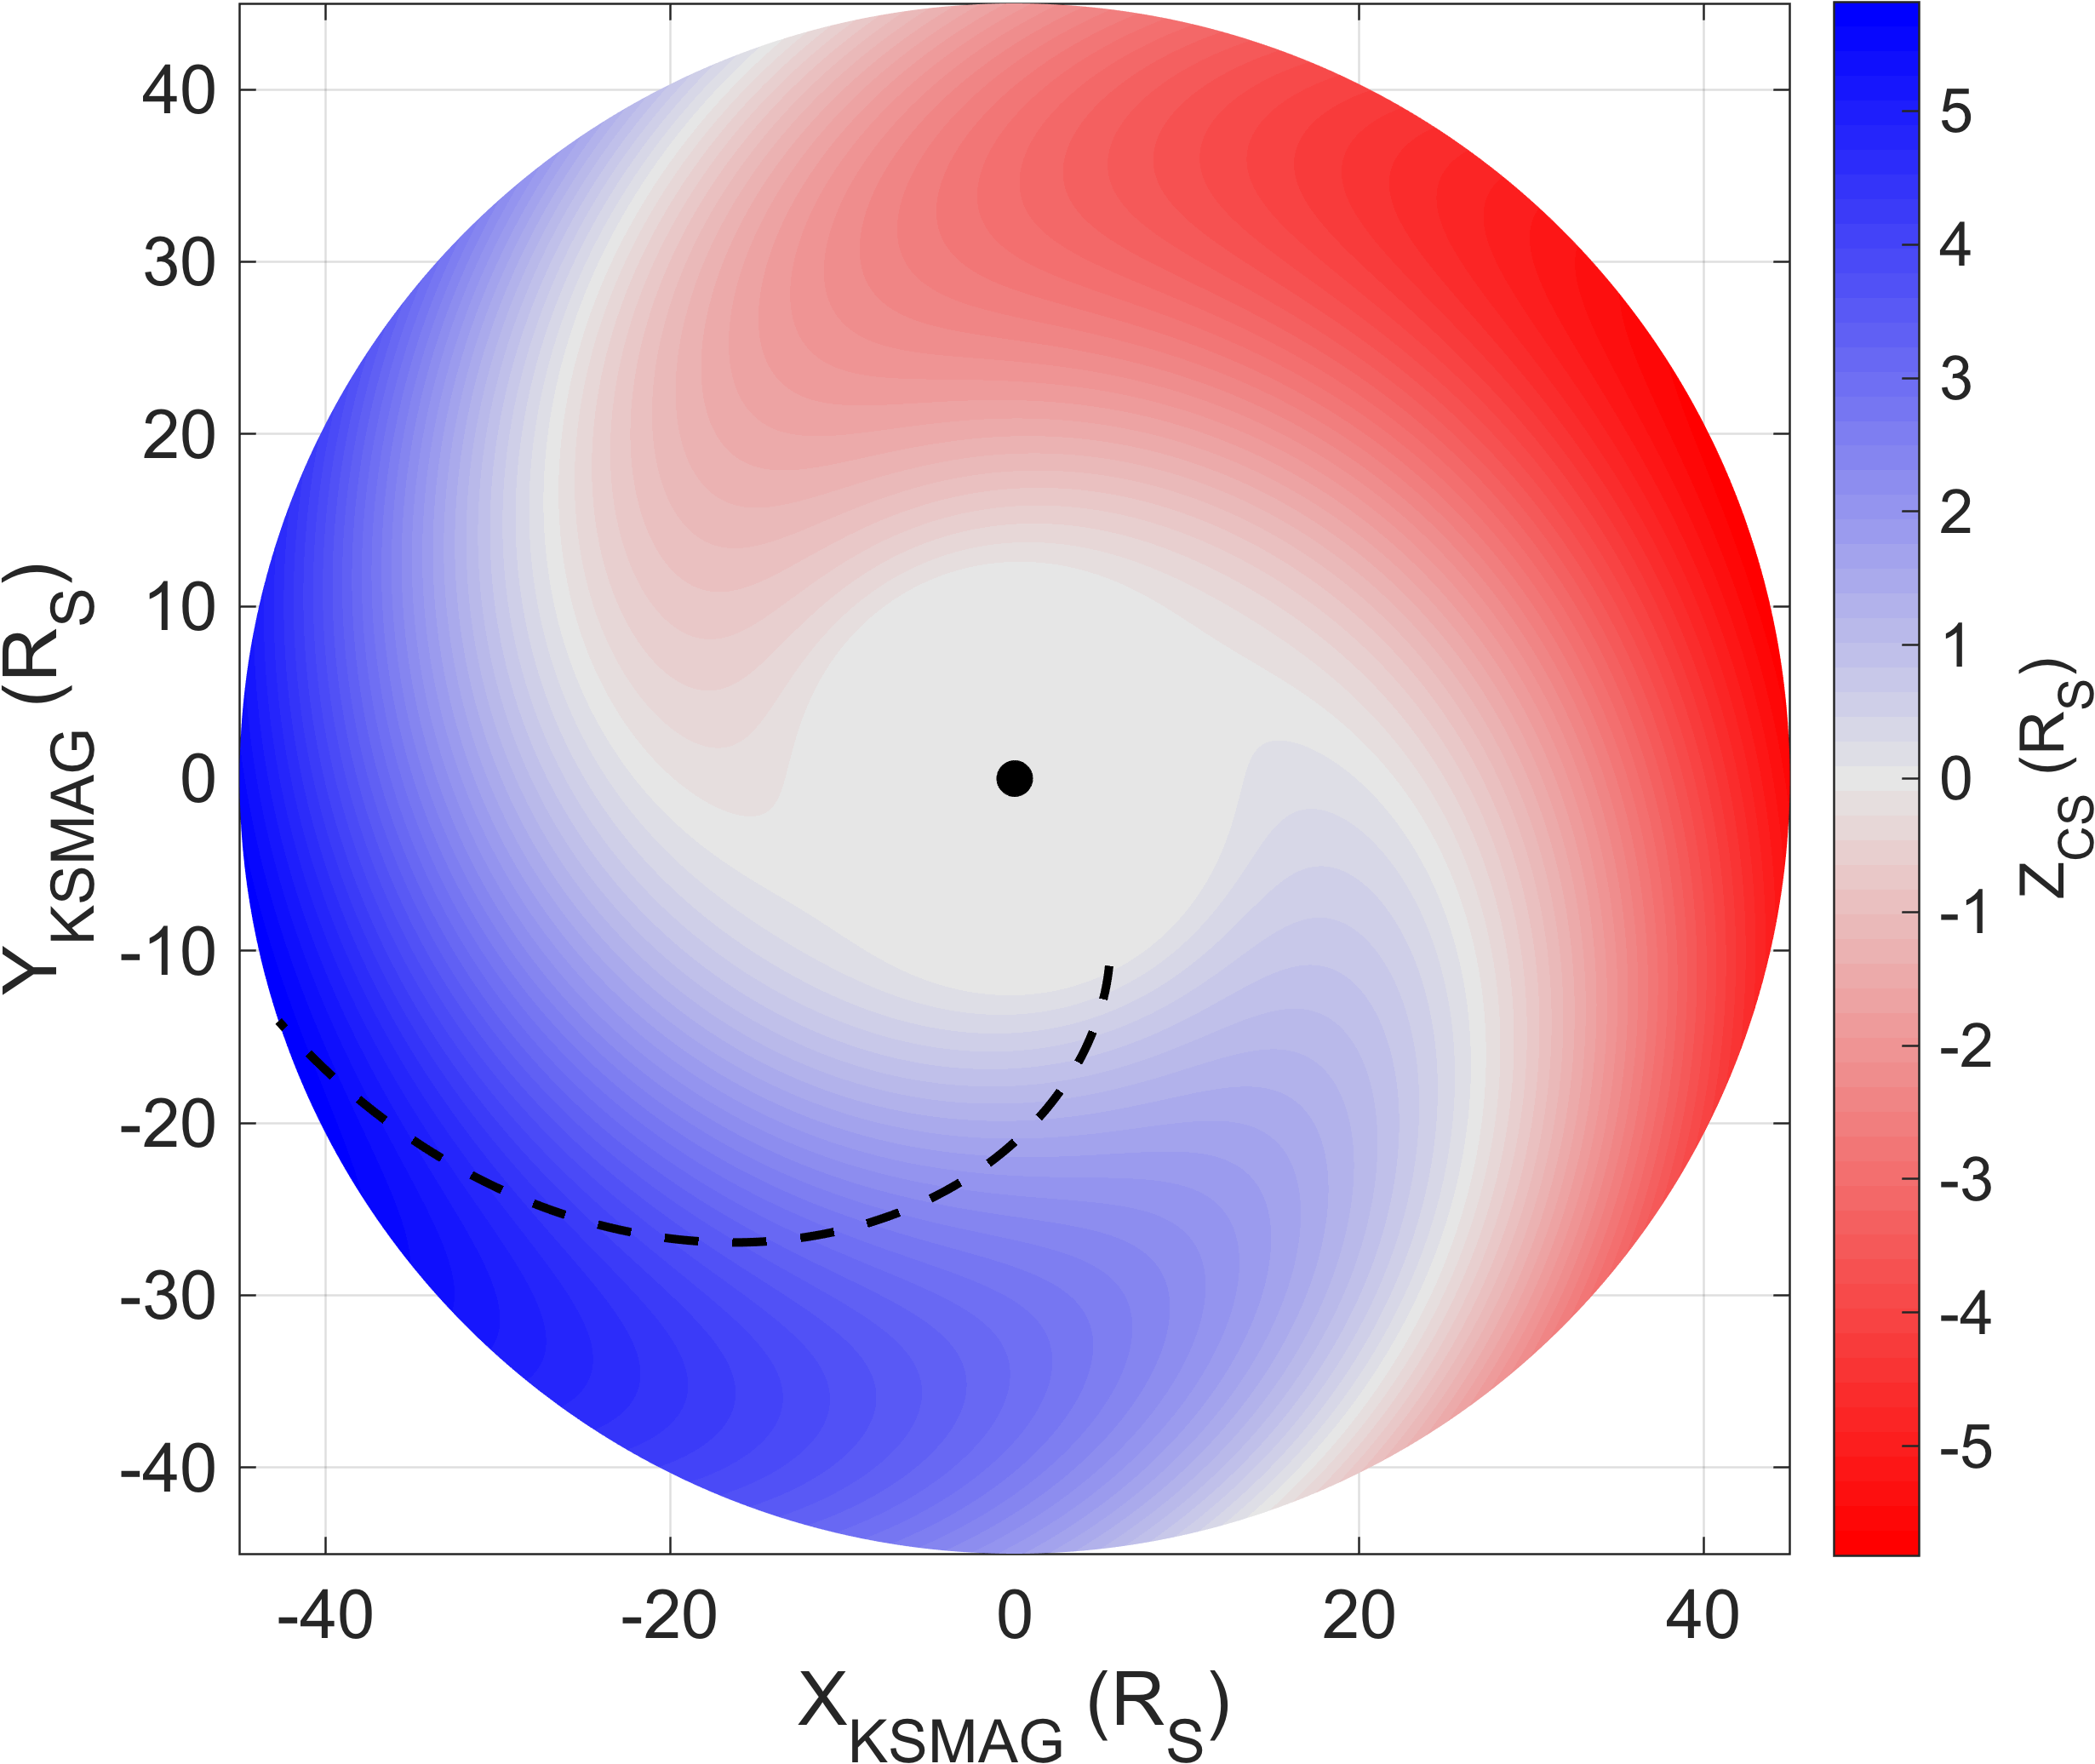
\includegraphics[width=0.6\textwidth]{equinox/cssurface.png}
% when using dvips, use .eps file:
% \includegraphics[width=20pc]{figsamp.eps}
\caption[Snapshot of tilted, rippled current sheet surface model.]{An snapshot of the current sheet surface model, with parameters $D~{=}~\SI{3}{\degree/R_S}$, $\theta_\mathrm{T}~{=}~\SI{10}{\degree}$, and $\rho_0~{=}~\SI{12}{R_S}$. Blue and red color indicates height of the current sheet $z_\mathrm{CS}$ above and below the rotational equator. The black dashed line represents a curve of constant phase $\lambda = \lambda_0$, passing through the maximum $z_\mathrm{CS}$ at each radial distance. The whole pattern then rotates with a variable period close to that of planetary rotation.}
\label{equinox:fig:cssurfacemodel}
\end{figure}

In the original study by \citet{arridge2011} the authors found values of $D$ varying from $2.1-\SI{6.7}{\degree/R_S}$ from orbit to orbit, with an average of $\SI{3.7}{\degree/R_S}$. This is in broad agreement with the results from \citet{carbary2007}, who looked for evidence of a spiral pattern in electron intensities directly using data from \textit{Cassini's} MIMI/LEMMS instrument (Magnetosphere Imaging Instrument/Low Energy Magnetospheric Measurement System) \citep{krimigis2004}. They observed an average `spiral arm migration' of ${{\sim}}\SI{3.4}{\degree/R_S}$, with a range of $2.7-\SI{4.7}{\degree/R_S}$. In the study by \citet{provan2012}, the authors analyze \textit{Cassini} magnetic field data from a similar time period, to measure how the phase of the magnetic perturbations discussed in the aforementioned \citet{andrews2012} study varies with radial distance and local time, specifically for the southern perturbation. They find a roughly constant radial phase gradient of ${{\sim}}\SI{2.5}{\degree/R_S}$. On the modeling side, \citet{jiaandkivelson2012} used their MHD model of Saturn's magnetosphere with twin atmospheric vortical flows to stimulate current sheet flapping (as discussed in Section~\ref{equinox:sec:intro}), and used the modeled current sheet location at different phases and radial distances to estimate a delay of ${\sim}\SI{4.3}{\degree/R_S}$. Therefore in line with these studies, we use a value of $D = \SI{3}{\degree/R_S}$ here, corresponding to a value $v_\mathrm{W} \approx \SI{185}{\km\per\second}$.

In reality, the appropriate parameter $D = \Omega_\mathrm{S}/v_\mathrm{W}$ would vary with radial distance and local time, as the wave velocity $v_\mathrm{W}$ is dependent on plasma parameters and magnetic field strength, which vary throughout the equatorial magnetosphere. Indeed \citet{andrews2010}, using \textit{Cassini} magnetic field data estimated a radial phase speed that varied from ${\sim}\SI{150}{\km\per\second}$ on Saturn's nightside to ${\sim}\SI{500}{\km\per\second}$ on the dayside, corresponding to $D$ varying from ${\sim}3-\SI{1}{\degree/R_S}$, although they qualify that the dayside value in particular has a high uncertainty. They note that this is at least in broad agreement with estimates based on measurements presented in \citet{wilson2008} and \citet{mcandrews2009}, which suggest typical Alfv\'{e}n speeds within the equatorial ring current region of ${\sim}100-\SI{400}{\km\per\second}$, depending on magnetospheric parameters. This would correspond to a delay parameter that varies between approximately $D = 6-\SI{1}{\degree/R_S}$ (where a higher value of $D$ corresponds to a lower value of $v_\mathrm{W}$). We investigated the effect of a variation in $D$ with radial distance of this scale but found it did not significantly influence our results compared to other factors. %In addition, allowing $D$ to vary as a free parameter created a degeneracy with the parameter $\lambda_0$, as both parameters influence the phasing of the magnetic field oscillations, and meant we could not extract meaningful values for either parameter.

\subsection{Magnetic Field and Plasma Model}\label{equinox:sec:plasmamodel}
The current sheet model geometry described in the previous section must be combined with a local model of magnetic field and plasma sheet structure in order to predict magnetic field values at \textit{Cassini} locations. We then geometrically `anchor' a magnetic field and plasma model to our perturbed current sheet surface model following the approach of \citet{achilleos2014}, described in that study and repeated below. We use a modified version of the model described by \citet{achilleos2010a}, itself based on a model originally constructed for the Jovian magnetodisk by \citet{caudal1986}, adapted for the Saturn system. More information can be found in those studies. The model is axisymmetric about the planetary dipole / rotation axis, which are assumed to be parallel. It is constructed based on the assumption of force balance in the rotating plasma of the magnetosphere between the Lorentz body force (magnetic pressure and tension forces), pressure gradient force and centrifugal force, such that
\begin{equation}\label{equinox:eq:forcebalance}
\boldsymbol{J} \times \boldsymbol{B} = \nabla P - nm_i\omega^2\rho\boldsymbol{\hat{\rho}}
\end{equation}
where $\boldsymbol{J}$ is the current density, $\boldsymbol{B}$ is the magnetic field vector and $\rho$ is cylindrical radial distance from the rotation / dipole axis, with $\boldsymbol{\hat{\rho}}$ its unit vector. The plasma properties are isotropic pressure $P$, ion number density $n$, mean ion mass $m_i$ and angular velocity $\omega$. A limitation of using a single mean ion mass along each individual field line is that the model cannot account for fine structural variation in magnetodisk thickness, caused by the concentration of heavier water ions towards the equatorial plane \citep[e.g.][]{persoon2009, nemeth2011}; other limitations are discussed in detail in \citet{achilleos2010a}. However, as demonstrated in that study, and \citet{achilleos2010b, sergis2018}, the model can accurately reproduce global average trends observed in Saturn's magnetodisk. This model is therefore demonstrably adequate for reproducing the relatively large-scale amplitude oscillations in the magnetic field data that are analyzed in this study.

By representing the magnetic field as the gradient of a magnetic Euler potential $\alpha$, equation (\ref{equinox:eq:forcebalance}) corresponds to a partial differential equation which can be solved iteratively for $\alpha$, providing magnetic field and plasma distributions as a function of cylindrical radial distance $\rho$, and height with respect to the rotational equator $z$.

We then extract magnetic field values from this model along \textit{Cassini} trajectories to directly compare with magnetometer data. The appropriate coordinates $\rho_\mu$ and $z_\mu$ at which to sample from this model are determined for each \textit{Cassini} sampling time by the current sheet model location $z_\mathrm{CS}$, according to
\begin{align}\label{equinox:eq:coordinatetransform}
& \rho_\mu = \rho_\mathrm{S/C},\nonumber\\
& z_\mu = (z_\mathrm{S/C} - z_\mathrm{CS})\hat{\boldsymbol{z}}\cdot\hat{\boldsymbol{n}}
\end{align}
where the subscript S/C refers to the \textit{Cassini} spacecraft's actual location, $\hat{\boldsymbol{z}}$ is the unit vector along the rotation / dipole axis, and $\hat{\boldsymbol{n}}$ is the unit vector normal to the model current sheet surface calculated according to equation~\ref{equinox:eq:zcs}, using $\rho = \rho_\mathrm{S/C}$ and the $\lambda$ value of the spacecraft location at that time.

The vector components of the magnetic field perturbation (total magnetic field minus the internal dipole) $\Delta B_i$ extracted from the model at these coordinates are then transformed back to give the predicted external magnetic field $\boldsymbol{B_\mathrm{ext}}$ via
\begin{equation}\label{equinox:eq:Bext}
\boldsymbol{B_\mathrm{ext}} = \Delta B_\rho \hat{\boldsymbol{\rho}}_\mathrm{CS} + \Delta B_z \hat{\boldsymbol{n}} + \Delta B_\phi \hat{\boldsymbol{\phi}}_\mathrm{CS}
\end{equation}
where
\begin{align}\label{equinox:eq:vectortransform}
& \hat{\boldsymbol{\rho}}_\mathrm{CS} = \frac{\hat{\boldsymbol{\phi}} \times \hat{\boldsymbol{n}}}{| \hat{\boldsymbol{\phi}} \times \hat{\boldsymbol{n}}|}, \nonumber\\
& \hat{\boldsymbol{\phi}}_\mathrm{CS} = \hat{\boldsymbol{n}} \times \hat{\boldsymbol{\rho}}_\mathrm{CS}
\end{align}
such that $\hat{\boldsymbol{\rho}}_\mathrm{CS}$ and $\hat{\boldsymbol{\phi}}_\mathrm{CS}$ lie in the local tangent plane of the model current sheet surface, while $\hat{\boldsymbol{\phi}}$ is in the direction of planetary corotation. As the model used here is purely poloidal we use $\Delta B_\phi = -\frac{1}{2} \Delta B_\rho$ to characterize the azimuthal magnetic field line bendback, again following \citet{achilleos2014}, adapted from the approach by \citet{arridge2011}. The internal magnetic field, represented by a dipole situated at Saturn's center, is then added to this external field to give the total magnetic field at that location. 

This formulation effectively assumes that the local magnetodisk structure at \textit{Cassini's} location may be approximated by the azimuthally symmetric \citet{achilleos2010a} plasma and magnetic field model, but with the equatorial plane of this model rotated to align with the local tangent plane of the model current sheet surface according to equation~\ref{equinox:eq:zcs}. More details can be found in {\citet{achilleos2014}}, who describe the transformation between the `model coordinates' used in the computation of the model field, and a local system of coordinates defined by the tangential plane of that part of the current sheet close to the spacecraft.

\subsubsection{Model Parameterization}\label{equinox:sec:modelparamzation}
The \citet{achilleos2010a} model treats the plasma as consisting of a cold population, confined towards the rotational equator due to the centrifugal force exerted on it, and a hot population with associated pressure distributed uniformly along magnetic field lines. The hot plasma population therefore can be completely characterized by a particular equatorial plasma pressure $P_\mathrm{H0}$ (the subscript 0 means the quantity evaluated at the equatorial crossing point of the magnetic field line) and flux tube volume $V$ per unit of magnetic flux, where
\begin{equation}\label{equinox:eq:ftv}
V = \int_{0}^{s_{B}} ds/B,
\end{equation}
and $ds$ is an element of arc length along the magnetic field line. The integral limits represent measurement along a field line of total length $s_B$ between the southern and northern ionospheric footprints at $\SI{1}{R_S}$.

Studies using \textit{Cassini} MIMI data, such as \citet{sergis2007, sergis2010}, have shown that the equatorial pressure associated with the hot plasma population is highly variable, with radial distance and over time. In light of these observations the original \citet{achilleos2010a} model simply parameterized the global hot plasma content, by assuming a profile such that in the middle and outer magnetosphere $P_\mathrm{H0}V = K_\mathrm{H}$ and $K_\mathrm{H}$ is a constant, known as the `hot plasma index'. Observations described in that study indicate that this index may vary in the range $10^5{\--}10^7~\si{\pascal\m\per\tesla}$. In the inner magnetosphere, inside $\SI{8}{R_S}$, the hot plasma pressure profile was constructed to decrease linearly with decreasing $\rho$, such that $P_\mathrm{H0}(\rho) = P_\mathrm{H0}(\rho = \SI{8}{R_S})\times(\rho/8)$. A similar parameterisation was made in \citet{caudal1986}, who argued that for the Jovian system, under the expected conditions of rapid radial diffusion, the hot plasma would be transported isothermally. Further discussion and justification of this parameterization can be found in \citet{achilleos2010a}.

In this study we used a value of $K_\mathrm{H} = \SI{3e6}{\pascal\m\per\tesla}$, in agreement with the corresponding \textit{in situ} observations made during the period being studied here. This is demonstrated in Figure~\ref{equinox:fig:hotpressuremodel}, which shows 10-minute-averaged hot pressure moments calculated from \textit{Cassini} MIMI data along the trajectories being studied here, and model predictions of the equatorial hot pressure profile using different $K_\mathrm{H}$ values as described in the legend. A third-order polynomial fit of the MIMI data in log-linear space is also shown, in grey, to further illustrate the agreement between the overall trend of the data and the $K_\mathrm{H} = \SI{3e6}{\pascal\m\per\tesla}$ model calculations. It should be noted that, as mentioned previously, these \textit{Cassini} trajectories are not exactly equatorial but lie within $+0.3/\SI{-1.2}{R_S}$ of the rotational equator; however, the variation in pressure associated with transient conditions is much greater than the variation associated with vertical distance from the equator for this data set, and so a comparison with the equatorial model profiles is appropriate here. We consider the potential impact of this assumption on our results in more detail in Section~\ref{equinox:sec:results}.
\begin{figure}
\centering
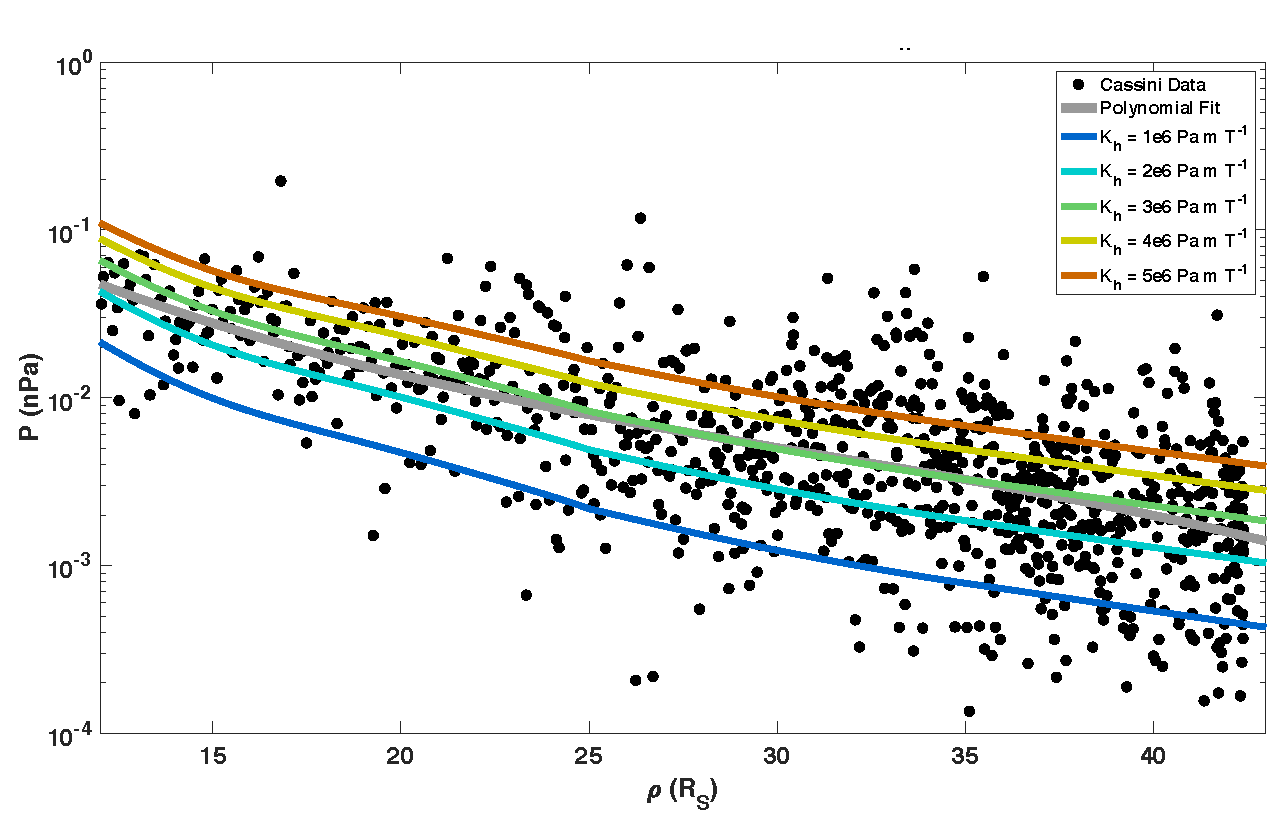
\includegraphics[width=0.8\textwidth]{equinox/hotpressuremodel.pdf}
\caption[Equatorial hot plasma pressure from \textit{Cassini} MIMI, and model predictions for different $K_\mathrm{H}$ values.]{Pressure distribution of the hot plasma population in Saturn's outer magnetosphere, against cylindrical radial distance $\rho$ in the KSMAG coordinate system. Black solid circles show 10 minute averaged hot plasma pressure moments calculated from \textit{Cassini} MIMI data along trajectories Revs 120-122, and colored lines show equatorial model profiles using values of $K_\mathrm{H}$ as shown in the legend. The grey line shows a third-order polynomial fit of the pressure data in log-linear space, as per the axes.}
\label{equinox:fig:hotpressuremodel}
\end{figure}

The model can also be parameterized by effective magnetodisk radius $R_\mathrm{D}$, which is the cylindrical radial distance from the origin to the last closed magnetic field line, representing the location of the magnetopause boundary in the equatorial plane. A value of $\SI{45}{R_S}$ was initially used in this study, representing a typical magnetopause boundary location on the dusk flank of the magnetosphere, where \textit{Cassini} spent the majority of its time during the trajectories being studied here. This choice is discussed in more detail in Section~\ref{equinox:sec:simulatingbreathing}.
%The effect of varying both of these parameters, $R_\mathrm{D}$ and  $K_\mathrm{H}$, on the global magnetodisk structure, are explored in detail in \citet{sorba2017}.

\subsubsection{Model modifications for this study}\label{equinox:sec:modmodifications}
As discussed at the beginning of this subsection, this model calculates the global magnetic field structure by iteratively solving a partial differential equation for the magnetic Euler potential $\alpha$, starting from a pure dipole solution and then successively perturbing it. At each iteration, a linear combination of the present solution $\alpha_i$ and the previous solution $\alpha_{i-1}$ is used as input for the next iteration calculation, such that
\begin{equation}
\alpha_{i+1\mathrm{(input)}} = \gamma\alpha_i + (1-\gamma)\alpha_{i-1},
\end{equation}
where $\gamma<1$ controls the relative weighting between the previous and current solutions. This is a form of numerical `relaxation'. This $\alpha_{i+1(\mathrm{input})}$ is then used in the partial differential equation, to solve for $\alpha_{i+1}$. In the original model construction, the two components were weighted equally ($\gamma=0.5$) and calculations continued until the maximum difference between successive iterations fell below a chosen `tolerance' $\delta = 0.5\%$. In this study we found that, for models with more extreme input parameters, (for example, large disk radii $R_\mathrm{D}$ but small hot plasma content $K_\mathrm{H}$ values), it was necessary to weight the previous solution up to four times more heavily than the present solution ($\gamma=0.2$), in order to approach convergence. In order to keep the ratio $\delta/\gamma$ constant at $10^{-2}$, and therefore consistent with our original approach, this corresponds to using a more stringent stopping tolerance $\delta = 10^{-2}\times0.2 = 0.2\%$ in such cases.

A small uniform southward-directed `shielding field' is also added to the magnetic field perturbation at every iteration, in order to account for the magnetic field associated with the magnetopause and magnetotail current sheets. In the original model construction, the magnitude of this field was chosen by calculating dayside equatorial averages of the empirical field models of \citet{alexeev2005} and \citet{alexeev2006}, and the value varied with model magnetodisk radius $R_\mathrm{D}$ \citep[see][Figure 6]{achilleos2010a}. In particular the component of the shielding field associated with the magnetopause currents was based on a dipole approximation of the magnetospheric magnetic field. However in this study, we calculate magnetodisk models with large $R_\mathrm{D}$ such that the global magnetic field structure deviates significantly from a dipolar configuration, and so the magnetic moment associated with the magnetodisc ring current is large compared to the planetary dipole magnetic moment. This can be quantified as the ratio of the ring current magnetic moment to planetary dipole magnetic moment $k_\mathrm{MD} > 1$. We therefore need to also account for the contribution of the magnetodisc magnetic moment to the magnetopause current. According to \citet{alexeev2005}, the magnitude of this contribution can be approximated to the zeroth order by the field associated with the dipole magnetopause current, multiplied by the ratio $k_\mathrm{MD}$, such that the total shielding field component associated with magnetopause currents is enhanced by the factor $(1+k_\mathrm{MD})$. Therefore in this study, for `large' models with $R_\mathrm{D} > \SI{30}{R_S}$ we modify the shielding field in this way, using an extrapolation of an empirical fit to \textit{Cassini} MAG data from \citet{bunce2007} to estimate $k_\mathrm{MD}$ for each magnetodisc radius. For example, for a model with $R_\mathrm{D} = \SI{40}{R_S}$, we use $k_\mathrm{MD}{\approx}1.3$ and find that this modification enhances the total shielding field in the southward direction by ${\sim}\SI{0.3}{nT}$. We found that a change of this order does not significantly affect the global magnetic field structure, but does improve the tendency for models with more extreme disk radii to achieve convergence.

The equatorial profile of plasma angular velocity $\omega$ is a boundary condition for this model, and was updated in this study to better represent the plasma behavior, particularly in the outer magnetosphere. The original profile was a sixth-order polynomial fit to azimuthal velocity measurements from studies by \citet{kane2008}, who used MIMI/INCA data, and \citet{wilson2008}, who used CAPS/INMS (Ion and Neutral Mass Spectrometer) data. This is shown by the blue line in Figure~\ref{equinox:fig:omegaprofile} (more detail in \citet{achilleos2010a}). We use more recent azimuthal velocity measurements from the study by \citet{wilson2017}. In that study the authors employ a more comprehensive CAPS data set, and an improved fitting technique, to derive median and upper/lower quartile values for equatorial azimuthal velocity in $\SI{0.5}{R_S}$ radial bins between 5 and $\SI{30}{R_S}$. These values, converted to angular velocities as a fraction of corotation using a planetary rotation rate $\Omega_S = \SI{1.6185e-4}{\radian\per\second}$ ($\SI{10.7833}{\hour}$ period), are shown by the black solid circles and error bars in Figure~\ref{equinox:fig:omegaprofile}. We fit the median values of azimuthal velocity with a fourth-order polynomial, with each point weighted by the error (assumed to be half of the interquartile range), to construct an equatorial angular velocity profile. The resulting profile used in this study is shown by the green line in Figure~\ref{equinox:fig:omegaprofile}, and polynomial coefficients with errors are given in the Appendix. We assume the plasma is in ideal corotation inside $\SI{4.5}{R_S}$, and constant plasma angular velocity beyond $\SI{29}{R_S}$ equal to the value at that point, to ensure a continuous profile. For a model with $R_\mathrm{D} = \SI{45}{R_S}$, we find that this profile slightly increases the total equatorial magnetic field strength in the inner and middle magnetosphere, and slightly decreases the equatorial magnetic field strength in the outer magnetosphere, and equal at around $\rho\approx\SI{35}{R_S}$. The most extreme difference from the original magnetic field strength profile was ${\sim}\SI{1.3}{nT}$ at around $\rho\approx\SI{15}{R_S}$. Alternatively, we could have assumed that the angular velocity decreases as $1/\rho^2$ beyond $\SI{29}{R_S}$, such that total angular momentum is conserved; however we find that this has only a very small impact on the resulting equatorial magnetic field profile (less than $\SI{0.1}{nT}$ maximum difference for a $R_\mathrm{D} = \SI{45}{R_S}$ model, at the very outer edge of the magnetosphere) and thus such an approach would not change the conclusions of this study.

This equatorial profile is then used to calculate $\omega$ throughout the model space, as $\omega$ is assumed constant along magnetic field lines in this model, in line with Ferraro's isorotation theorem; more details can be found in {\citet{achilleos2010a,caudal1986}}.
\begin{figure}
\centering
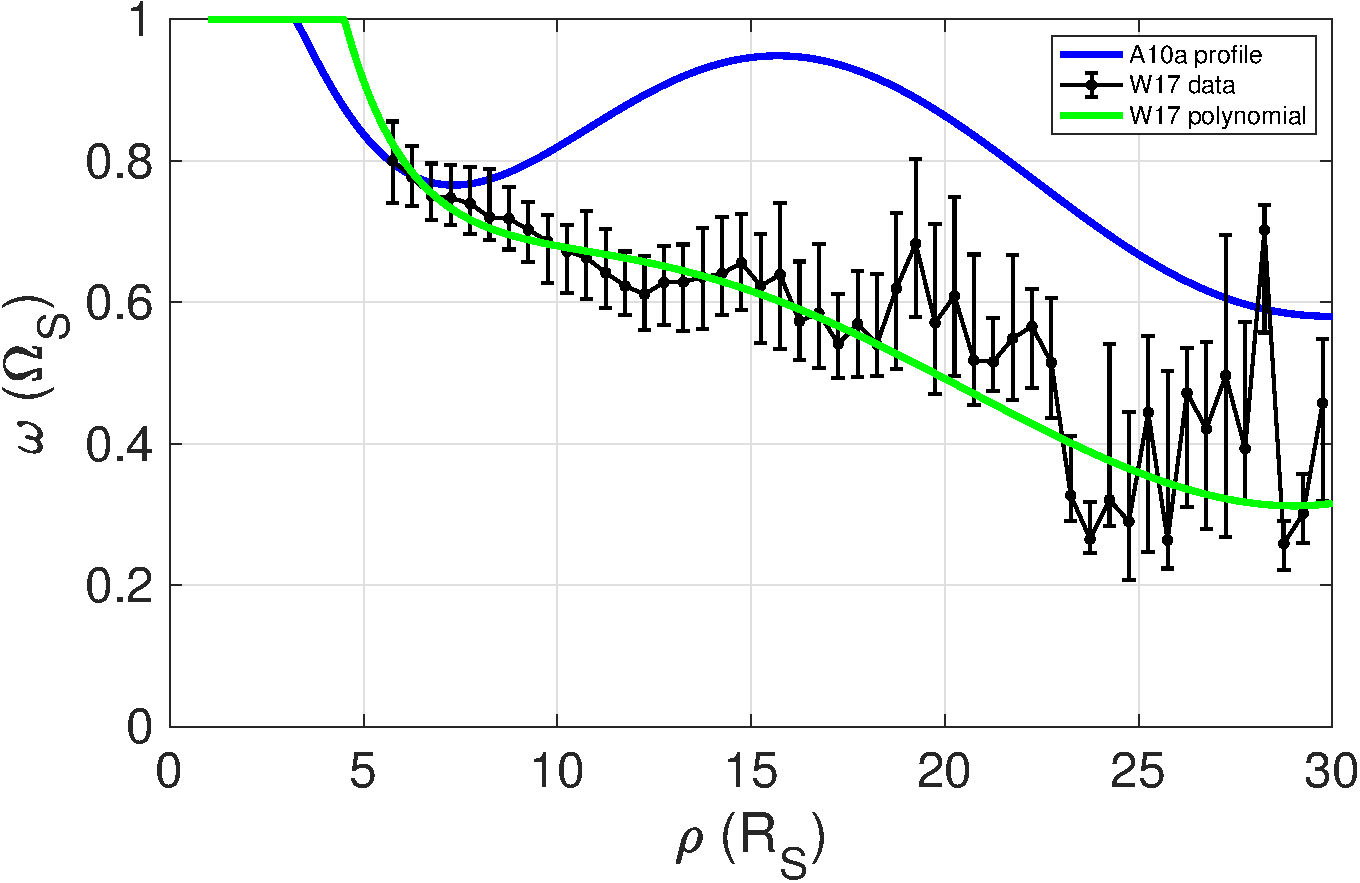
\includegraphics[width=0.7\textwidth]{equinox/omegaprofile.pdf}
\caption[Equatorial profile of plasma angular velocity from \citet{wilson2017}, with best fit polynomial.]{Plasma angular velocity at the equator as a fraction of planetary corotation, as a function of cylindrical radial distance. Black solid circles and error bars show the median and upper/lower quartile values of binned measurements of azimuthal velocity from \citet{wilson2017}, converted to angular velocity as described in the text. A fourth-order polynomial fit to these points, used in this study, is shown by the green line. The original angular velocity profile used in the \citet{achilleos2010a} model is shown by the blue line.}
\label{equinox:fig:omegaprofile}
\end{figure}

\subsection{Simulating the Breathing Behavior}\label{equinox:sec:simulatingbreathing}
As described in Section~\ref{equinox:sec:intro}, Saturn's magnetospheric current sheet is observed to not only periodically flap above and below the rotational equator, but also to periodically thicken and thin (`breathing'). In this study we attempt to simulate this compressional perturbation in a novel way, by modulating the magnetodisc radius $R_\mathrm{D}$ of the magnetic field and plasma model we sample from, depending on longitude. This is a departure from the study by {\citet{achilleos2014}}; those authors used a single magnetodisc model with a fixed value of $R_\mathrm{D}$ at all azimuths, and hence did not include the periodic modulation of the current sheet thickness in their model construction. In general a model with a larger disk radius has a thinner, more distended current sheet, with magnetic field lines more `stretched out' in the radial direction, due to force balance mainly between the magnetic tension and centrifugal forces \citep{achilleos2010a,sorba2017}. In contrast a model with a relatively small disk radius has a more dipolar magnetic field structure, with more compressed field lines, and a correspondingly thicker current sheet.

We use a maximum value for $R_\mathrm{D}$ at a phase of the perturbation determined by $\lambda_\mathrm{B}$, and a minimum value at the opposite phase $\lambda_\mathrm{B}+\SI{180}{\degree}$. We vary this harmonically such that the appropriate $R_\mathrm{D}$ to use at any phase $\lambda$ determined by equation~\ref{equinox:eq:lambda} is given by
\begin{equation}\label{equinox:eq:RD}
R_\mathrm{D} = \frac{1}{2}[ R_\mathrm{MAX}+R_\mathrm{MIN}+(R_\mathrm{MAX}-R_\mathrm{MIN})\cos{(\lambda - \lambda_\mathrm{B})}].
\end{equation}
$\lambda_B$ is therefore an offset parameter for the breathing perturbation, a `prime meridian' just as $\lambda_0$ is for the flapping perturbation. It is used to describe the phase of the maximum equatorial displacement of the magnetopause boundary, and therefore thinnest current sheet, and is measured relative to $\lambda$, which is equivalent to $\lambda_\mathrm{MS}$ at $\rho=\rho_0$. The entire breathing-related perturbation then follows a spiral pattern with radial distance due to the radial delay in the perturbation propagation, as for the flapping perturbation (see equation~\ref{equinox:eq:lambda}).

This approach is illustrated in Figure \ref{equinox:fig:harmonicRD}. Panel (a) shows how the model disk radius $R_\mathrm{D}$ (shown by the solid black line) varies in $\lambda$ phase space according to equation~\ref{equinox:eq:RD}, using values $R_\mathrm{MIN}=\SI{45}{R_S}$ and $R_\mathrm{MAX}=\SI{55}{R_S}$. It can be seen that the largest disk radius is used at $\lambda=\lambda_\mathrm{B}$, and the smallest at $\lambda=\lambda_\mathrm{B}+\SI{180}{\degree}$. Panel (b) shows how this then translates into real space for a given moment in time, with color representing which magnetodisc model radius $R_\mathrm{D}$ is used at each location.
\begin{figure}
\centering
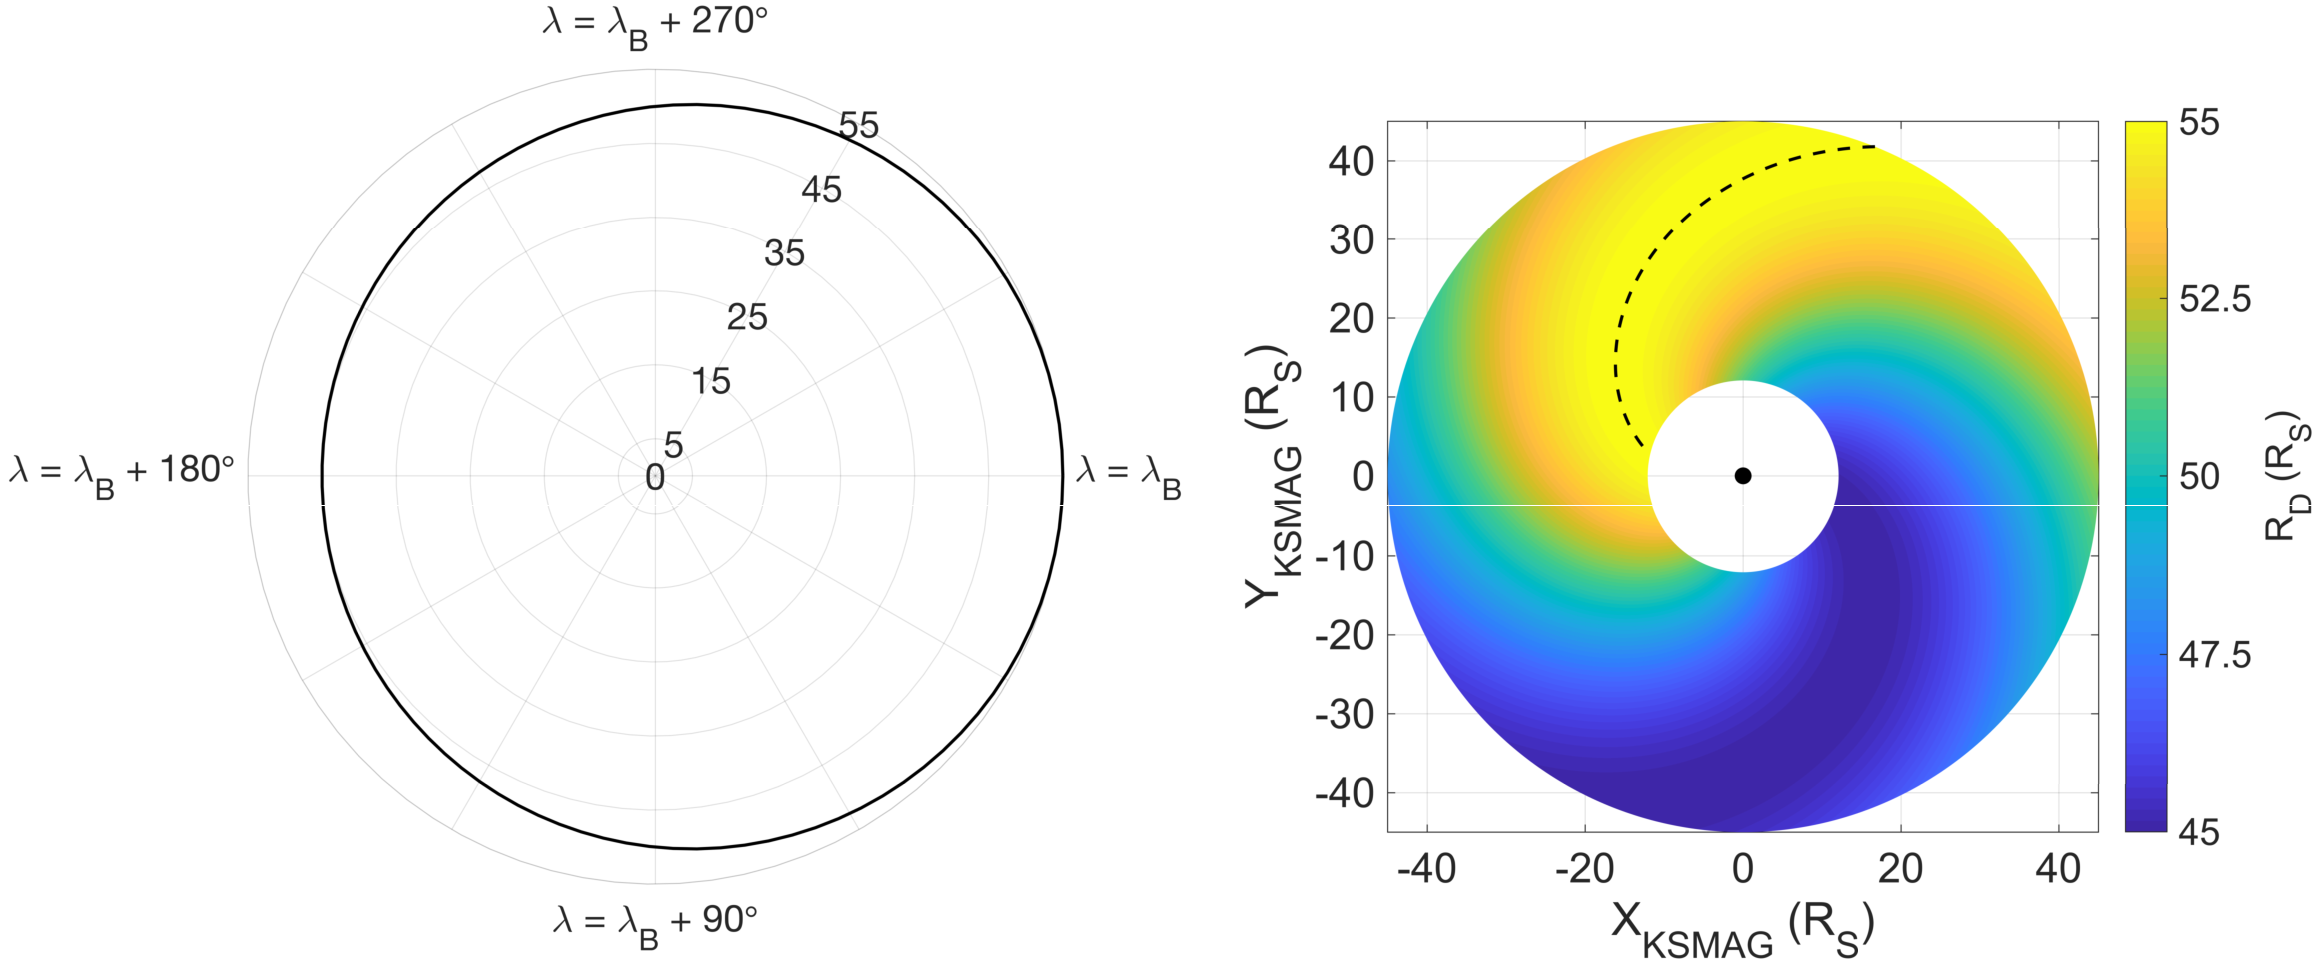
\includegraphics[width=0.9\textwidth]{equinox/harmonicRD.pdf}
\caption[Diagram showing how magnetodisc model radius $R_\mathrm{D}$ varies with phase, to represent breathing.]{(a) How the magnetodisc model radius $R_\mathrm{D}$ varies with phase $\lambda$, according to equation~\ref{equinox:eq:RD}. Black solid line shows $R_\mathrm{D}$, grey circles labeled with numbers from 0-55 show radius in units of $\si{R_S}$. (b) Translation of pattern (a) into real space at a given moment in time, according to $\lambda$ as described by equation~\ref{equinox:eq:lambda}. Color shows magnetodisc model radius $R_\mathrm{D}$ used at each location. The black dashed line highlights where $\lambda=\lambda_\mathrm{B}$, and hence a `breathing prime meridian' where the largest disk radius is used.}
\label{equinox:fig:harmonicRD}
\end{figure}

To determine appropriate values of $R_\mathrm{MIN}$ and $R_\mathrm{MAX}$, we compared the time period of \textit{Cassini} data being used in this study to the list of \textit{Cassini} magnetopause crossings provided by \citet{pilkington2015}. In particular, we found a period of 5 days (8 - 12 November 2009) where 24 magnetopause crossings were observed in very quick succession, each separated by only a few hours. As discussed in more detail in \citet{pilkington2015}, this suggests that the magnetopause was likely to be close to equilibrium over this time period, as otherwise only a small number of crossings would be observed as the magnetopause boundary moved rapidly over the spacecraft. We assume that the incident solar wind dynamic pressure was roughly constant over this time period, and that the observed perturbation in the magnetopause boundary location was at least in part due to changing internal pressure. This could potentially be associated with the compressional `breathing' magnetic perturbation that we are investigating here, and thus we use this perturbation in the magnetopause location to estimate a reasonable disk radius perturbation.

Figure~\ref{equinox:fig:crossingssurface} shows the locations of the observed magnetopause crossings in the KSM coordinate system, where $x_\mathrm{KSM}$ points towards the sun and $\rho_\mathrm{Y,ZKSM} = \sqrt(y_\mathrm{KSM}^2 + z_\mathrm{KSM}^2)$ is the perpendicular distance from this axis. Two potential magnetopause surface locations using the~\citet{pilkington2015} model are also shown, both using a value for solar wind dynamic pressure of $\SI{0.04}{nPa}$, and with a local plasma $\beta$ value of 0 for the inner model surface and 1.5 for the outer model surface, to replicate a change in boundary location due to internal pressure changes. These model surfaces were chosen to broadly encapsulate the range of magnetopause crossings in this time period, and thus estimate the corresponding variation in magnetopause radius. However it must be noted that these model surfaces do not represent unique solutions to the crossings shown here and are merely used to get an idea of the changing magnetopause location for this period.
\begin{figure}
\centering
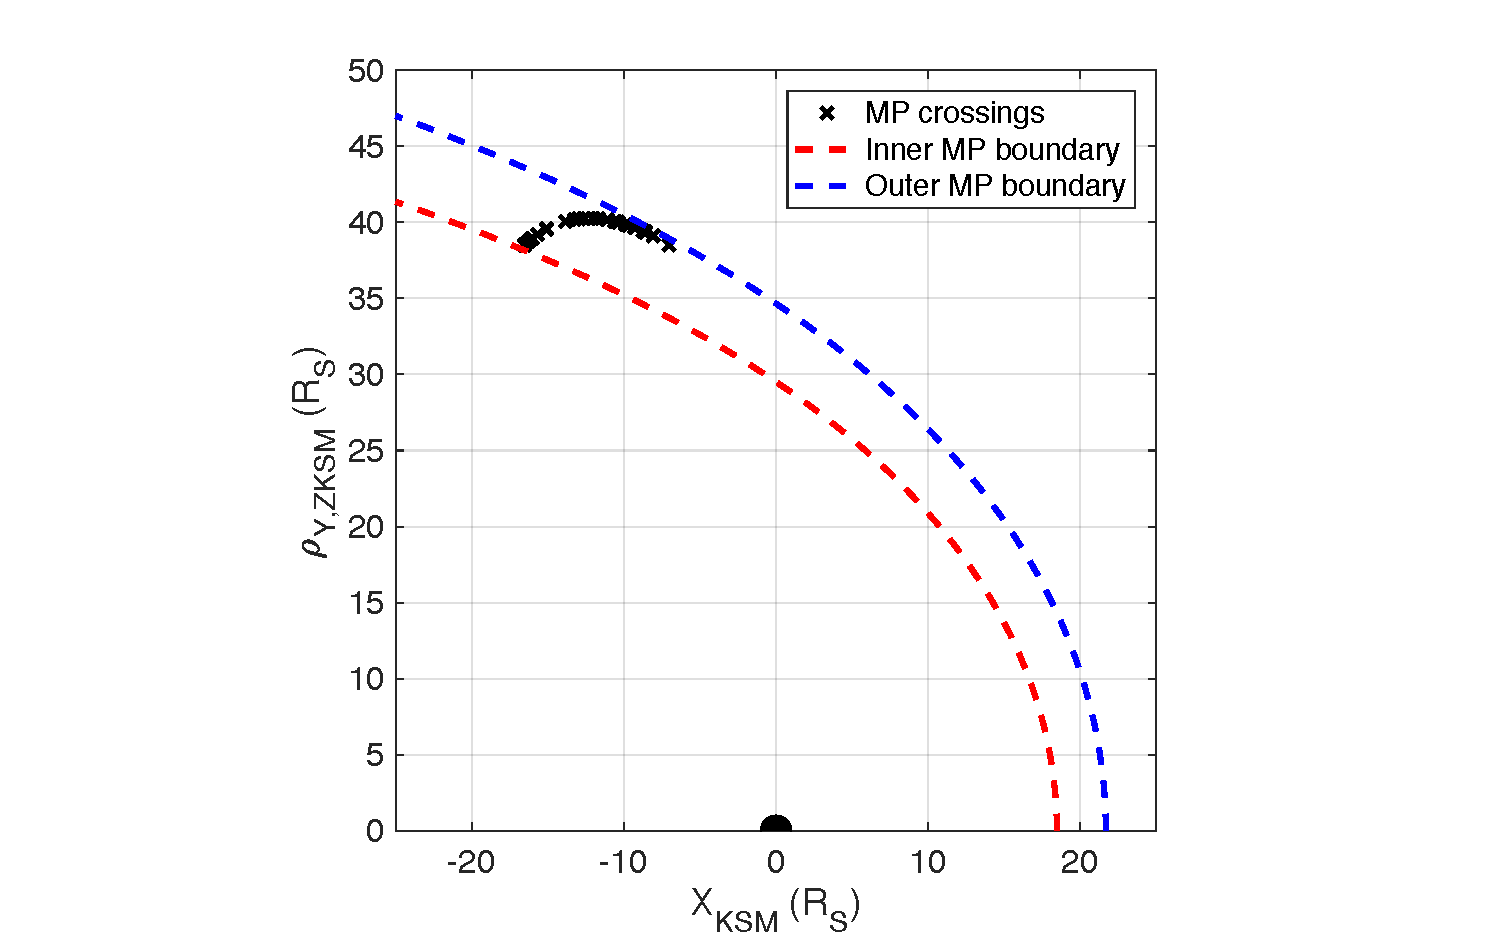
\includegraphics[width=0.5\textwidth]{equinox/crossingssurface.pdf}
\caption[Magnetopause crossings observed by \textit{Cassini}, and model magnetopause surfaces.]{Magnetopause crossings observed by \textit{Cassini} in the period 8 -12 November 2009, from \citet{pilkington2015}, in the KSM coordinate system. Model surfaces from the same study are shown in red and blue, using values for solar wind dynamic pressure and local plasma $\beta$ as described in the main text. Saturn is shown to scale at the origin by the black semicircle.}
\label{equinox:fig:crossingssurface}
\end{figure}

The difference in magnetopause radius of the two magnetopause model surfaces is $21.7-18.5 \approx\SI{3}{R_S}$ at the magnetopause nose. At the dusk flank, along the radial vector pointing from Saturn to the most anti-sunward crossing, this difference increases to $48.3-41.1\approx\SI{7}{R_S}$. A similar and even greater scale of perturbation was observed by \citet{clarke2010}, who analyzed \textit{Cassini} magnetic field and plasma electron data and found evidence that the magnetopause boundary oscillates by ${\sim}1.2{\--}\SI{5}{R_S}$ at the magnetopause nose, with a period close to the planetary rotation rate due to some internal rotating perturbation. In \citet{kivelson2014} the authors show that an MHD model that accurately predicts the current sheet flapping also produces a perturbation of ${\sim}\SI{5}{R_S}$ in the nose magnetopause location. In general a given radial perturbation in the magnetopause subsolar location corresponds to a ${\sim}2\times$ greater perturbation at the flank, using a \citet{pilkington2015} style model.

In light of these observations, and our requirement that the minimum model disk radius $R_\mathrm{D} \gtrsim \SI{44}{R_S}$ in order to provide coverage for our entire \textit{Cassini} data set, we use $R_\mathrm{MIN} = \SI{45}{R_S}$ and $R_\mathrm{MAX}=\SI{55}{R_S}$. This perturbation of $\SI{10}{R_S}$ is chosen to simulate the perturbation in the magnetopause boundary particularly on the dusk flank, where \textit{Cassini} spends most of its time for the trajectories being studied here (see Figure~\ref{equinox:fig:cassinitrajectory}). We calculate a family of five reference models with $R_\mathrm{D}$ linearly spaced in this range, and piece-wise linearly interpolate magnetic field values for the required $R_\mathrm{D}$ between them, thus assuming that the model magnetic field components at a given $\rho,z$ vary piece-wise linearly with global magnetodisc size $R_\mathrm{D}$. Figure~\ref{equinox:fig:MDALLcsthickness} (a)-(c) shows plots of how the hot plasma pressure $P_\mathrm{H}$ varies in cylindrical coordinates $\rho$ and $z$ for three of the five models we use in this study. As this quantity $P_\mathrm{H}$ is constant along magnetic field lines, this effectively shows the magnetic field structure for each of the magnetodisc models. A reference line at $z=\SI{4}{R_S}$ is included to show that for the larger magnetodisc model with $R_\mathrm{D}=\SI{55}{R_S}$, the current sheet is thinner and the magnetic field structure is more disk-like than for the models with smaller $R_\mathrm{D}$. Figure~\ref{equinox:fig:MDALLcsthickness} (d) shows equatorial magnetic field profiles for the five models used in this study. The similarity between the different profiles illustrates that our approach, of linearly interpolating between them to represent outputs from models with intermediate disk radii, is broadly appropriate here.

In reality, the thickness of Saturn's magnetospheric current sheet also varies with local time, with, in general, a thicker and more compressed current sheet on the dayside than the nightside \citep[e.g.][]{arridge2008}. In order to accurately account for this behavior, the value of $R_\mathrm{D}$ could be also varied as a function of local time, or the family of magnetodisc models could be otherwise modified to more accurately represent different local time sectors. While non-trivial and beyond the scope of this current study, we would like to investigate this in future, potentially using recent comprehensive results from \citet{sergis2017} as inputs to the \citet{achilleos2010a} model in order to more accurately represent local time variations in magnetodisc structure. However, for this study, our current approach is appropriate in this context and unlikely to significantly affect our conclusions. This is because we analyze each \textit{Cassini} pass individually, and the range in local time for each pass is only $\sim2-3.5$ hours, as shown by the annotations at the bottom of Figures~\ref{equinox:fig:rev120in}{\--}\ref{equinox:fig:rev122out}. This means that any variation in current sheet thickness associated with local time is likely to be less significant than the variation due to the magnetodisc breathing behavior.
\begin{figure}
\centering
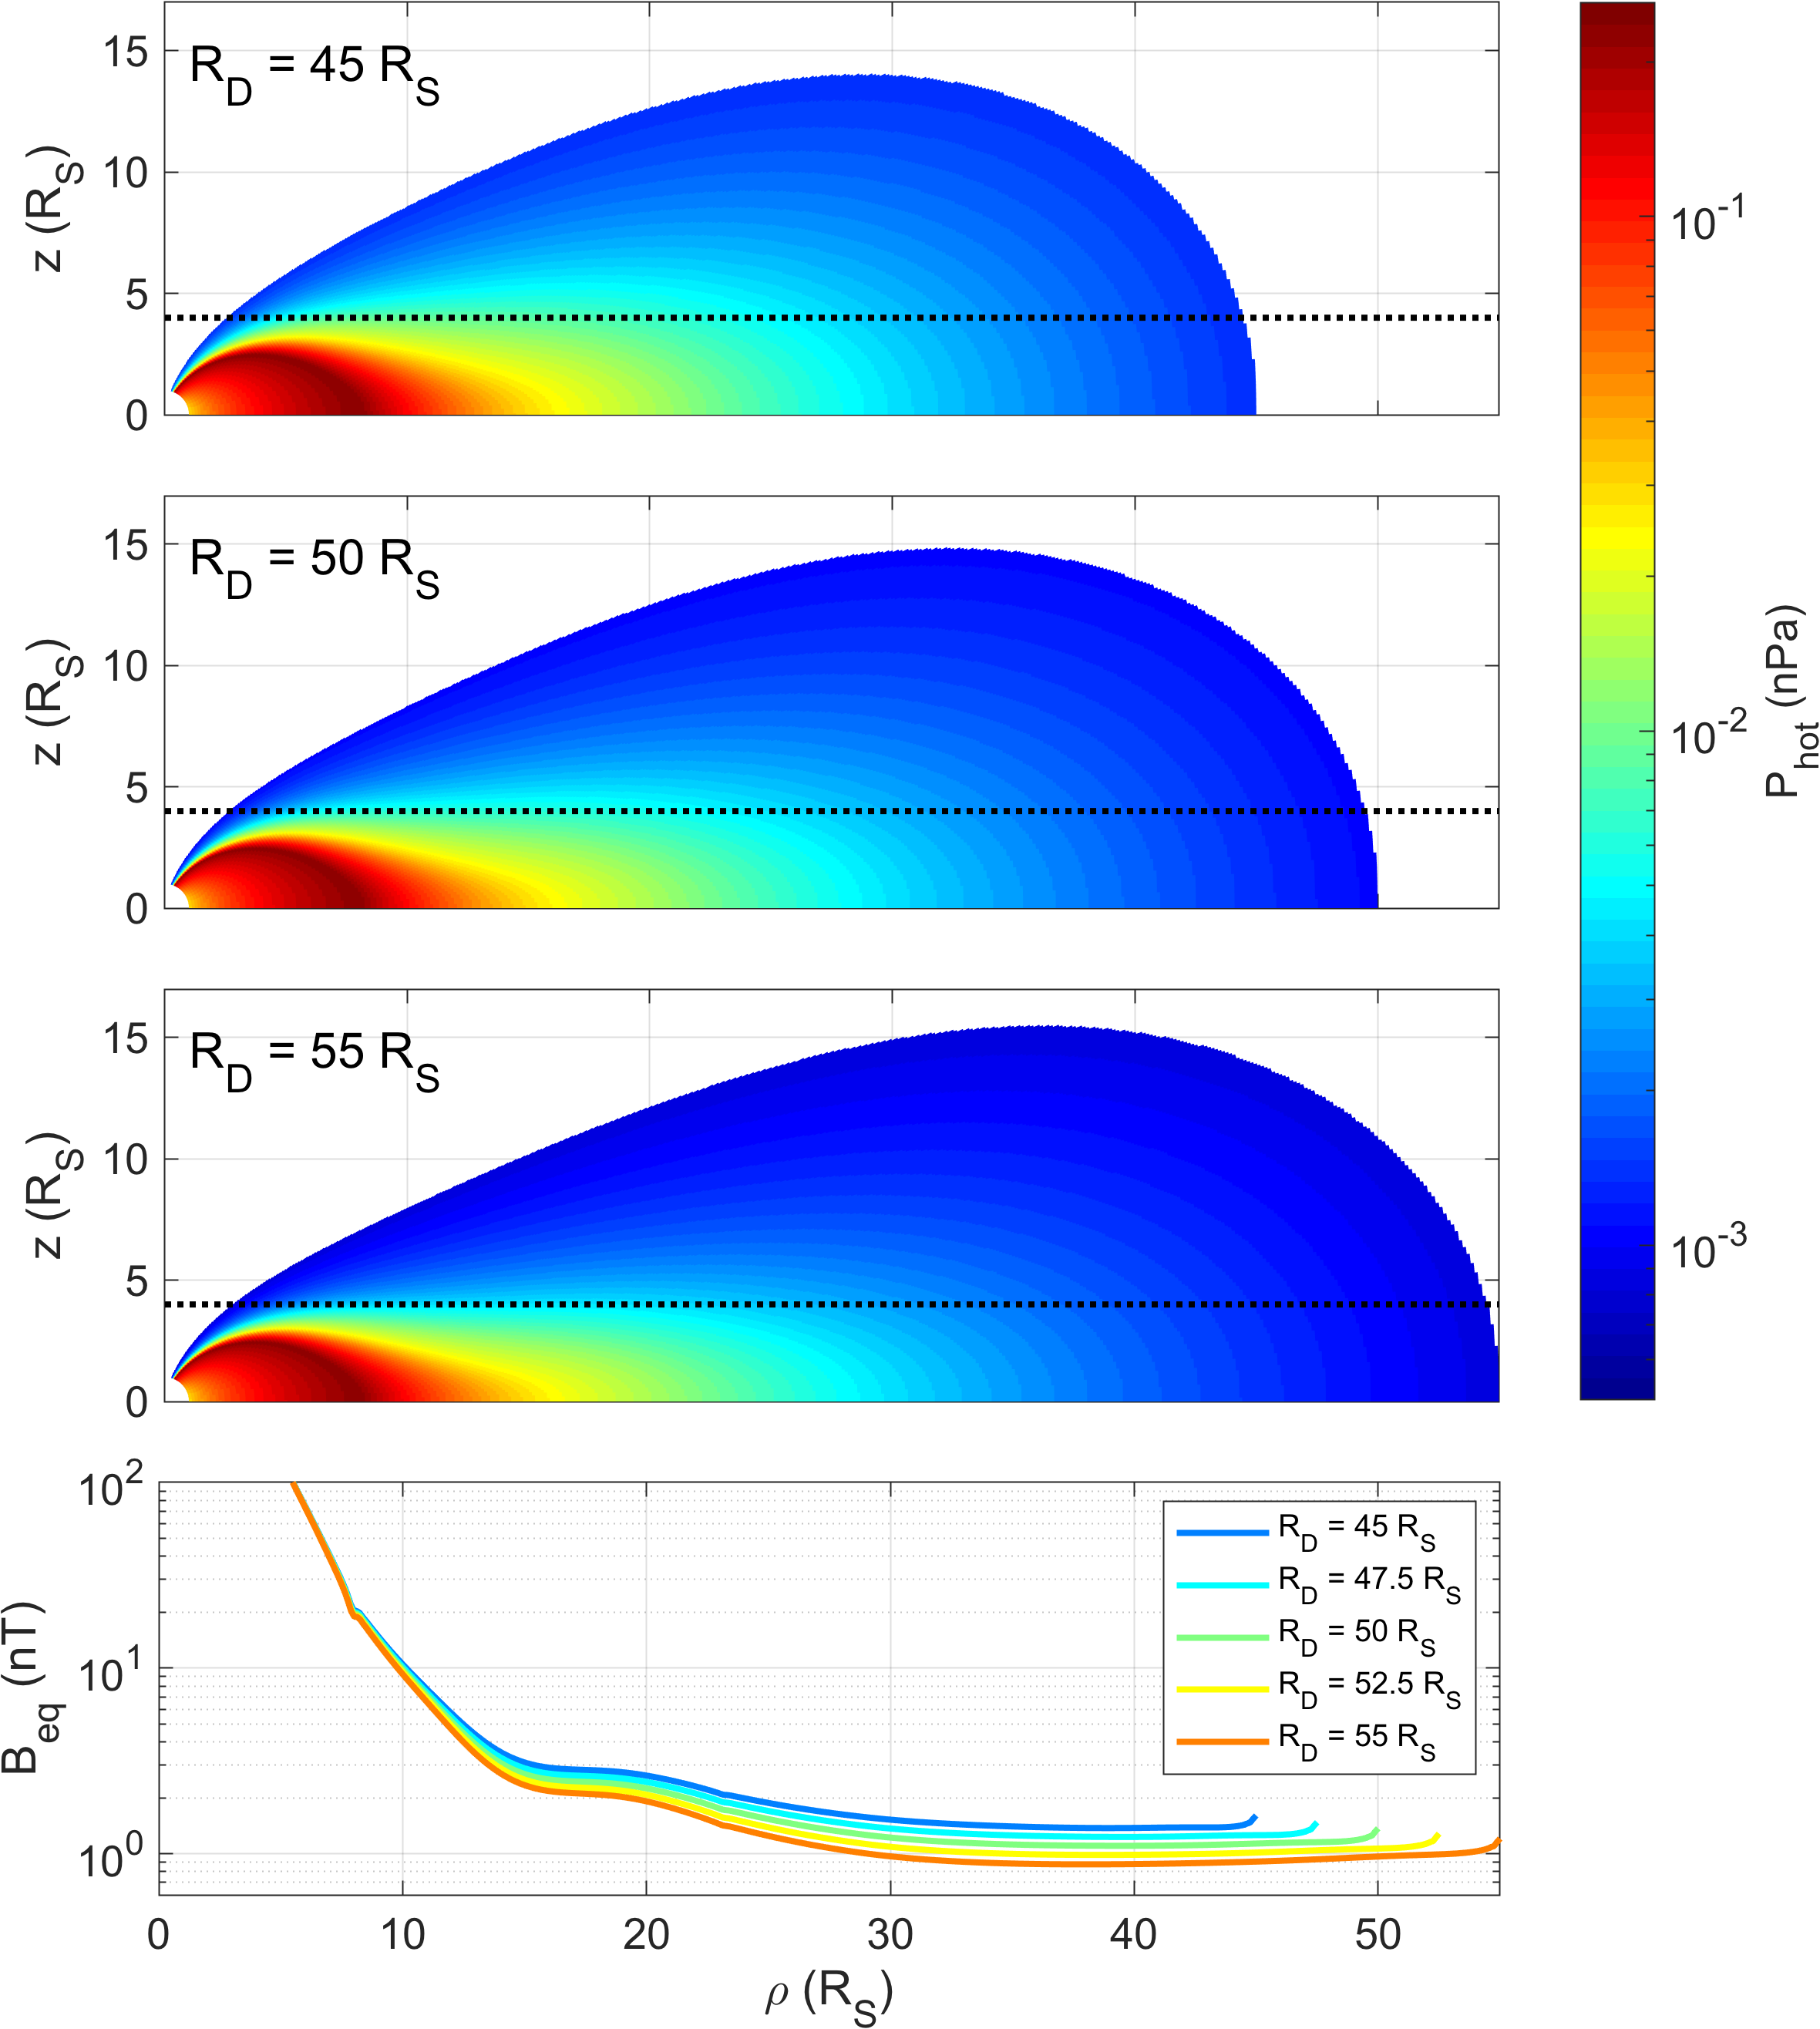
\includegraphics[width=0.6\textwidth]{equinox/MDALLcsthickness_Bfield.png}
\caption[Magnetic field structure for $R_\mathrm{D}$ = $45, 50$ and $\SI{55}{R_S}$ magnetodisc models.]{(a)-(c) Hot plasma pressure $P_\mathrm{H}$ predicted by the magnetodisc models as a function of cylindrical coordinates $\rho$ and $z$, shown on a color scale as per the colorbar. Models calculated using model disk radii $R_\mathrm{D}$ (a) $\SI{45}{R_S}$, (b) $\SI{50}{R_S}$ and (c) $\SI{55}{R_S}$. The quantity $P_\mathrm{H}$ is constant along a given magnetic field line and thus contours are equivalent to magnetic field lines. Black dotted line at $z~{=}~\SI{4}{R_S}$ is superimposed on each plot for reference, to compare current sheet thicknesses for each model. (d) Radial profiles of equatorial magnetic field strength for each of the five models used in this study, as shown by the legend.}
\label{equinox:fig:MDALLcsthickness}
\end{figure}

\subsection{Fitting Method and Parameter Uncertainty Estimation}
We fit the model to all three components of the 1-hour averaged magnetic field vector data measured by \textit{Cassini} in spherical polar coordinates, with $\boldsymbol{\hat{\phi}}$ in the direction of planetary corotation, $\boldsymbol{\hat{r}}$ pointing radially away from the planet, and $\boldsymbol{\hat{\theta}}$ completing the right-handed set. We separate our \textit{Cassini} trajectories into inbound and outbound passes, and fit the current sheet model parameters relevant for each pass. For the `flapping only' model, we use a fixed magnetodisc radius $R_\mathrm{D} = \SI{45}{R_S}$ and fit the parameters $\theta_\mathrm{T}$ and $\lambda_0$, and for the `flapping and breathing' model we use a range of disk radii as described above, and fit $\theta_\mathrm{T}$, $\lambda_0$ and $\lambda_\mathrm{B}$. We use a standard non-linear least squares fitting method, minimizing the unweighted merit function
\begin{equation}
\chi^2 = \sum\limits_{i,k}(B_{k}-\hat{B_{k}})_i^2~~~~i = 1,...,N;~k = r,\theta,\phi
\end{equation}
effectively the sum of the squared differences between the model and data magnetic field vector components, where $B_k$ is the observed and $\hat{B_k}$ is the model vector component for each of the $N$ data points. We minimized this function using the Levenberg-Marquardt algorithm, and use the square root of the diagonal elements of the resulting covariance matrix to estimate the standard error, and thus 95 percent confidence limits on the fitted parameters, following \citet{press2007}.

\section{Results and Discussion}\label{equinox:sec:results}
\subsection{Results with Flapping Only, and With Influence of Breathing}
\begin{table}
\caption[Fitted parameters for FO and F{\&}B models, for \textit{Cassini} Revs 120-122.]{Tables showing fitted parameters $\theta_\mathrm{T}$, $\lambda_0$ and $\lambda_\mathrm{B}$ for each Cassini revolution (Rev) using the flapping only (`FO') model and the flapping and breathing (`F{\&}B') model. Also shown is the root-mean-square difference (RMS) between model and data magnetic field values, and the approximate phase difference between the Southern and Northern magnetic perturbations at the center time of each pass from \citet{andrews2012} (S-N). }\label{equinox:table:fitparams}
\centering
\begin{tabular}{l l c c c c | c}
%\hline\hline
\hhline{=======}
 Rev & Model & $\theta_\mathrm{T}~(\si\degree)$& $\lambda_0~(\si\degree)$ & $\lambda_\mathrm{B}~(\si\degree)$ & RMS ($\si{nT}$) & S-N ($\si{\degree}$) \\
%\hline\hline
\hhline{=======}
\multirow{2}{*}{120 IN}  		& FO  		& $17.0\pm2.4$ 	& $247\pm6$ 	& -						& 1.16 	&	\multirow{2}{*}{286}\\
  											& F{\&}B  	& $14.3\pm1.8$ 	& $244\pm6$ 	& $20\pm30$ 	& 1.06	&\\   \hhline{-------} %\hline
\multirow{2}{*}{120 OUT}	& FO 		& $5.0\pm1.3$ 		& $139\pm14$ 	& - 						& 0.82	& \multirow{2}{*}{237}\\
 											& F{\&}B 	& $3.6\pm1.0$ 		& $134\pm16$ 	& $310\pm40$ 	& 0.81 &\\ \hhline{-------} %\hline
\multirow{2}{*}{121 IN} 		& FO 		& $7.4\pm1.8$ 		& $5\pm13$ 		& - 						& 1.19 & \multirow{2}{*}{156} \\
  											& F{\&}B 	& $6.4\pm1.4$ 		& $11\pm12$ 	& $270\pm40$	& 1.12 & \\ \hhline{-------} %\hline
\multirow{2}{*}{121 OUT}	& FO 		& $10.4\pm2.0$ 	& $268\pm9$ 	& -						& 0.65 & \multirow{2}{*}{99}\\
											& F{\&}B 	& $8.4\pm1.2$ 		& $259\pm7$ 	& $191\pm22$ 	& 0.53 & \\ \hhline{-------} %\hline
\multirow{2}{*}{122 IN}		& FO 		& $14.9\pm2.5$ 	& $280\pm8$	& -						& 1.27 & \multirow{2}{*}{52} \\
											& F{\&}B 	& $18.4\pm2.3$ 	& $285\pm5$ 	& $200\pm30$ &	1.16 &\\ \hhline{-------} %\hline
\multirow{2}{*}{122 OUT}	& FO 		& $8.1\pm1.5$ 		& $205\pm10$ & -					& 0.90	& \multirow{2}{*}{10}\\
											& F{\&}B 	& $6.8\pm1.4$ 	& $202\pm11$ 	& $310\pm40$		&	0.97 &\\
%\hline\hline
%\hhline{=======}
\hhline{-------}
%\multicolumn{2}{l}{$^{a}$Footnote text here.}
\end{tabular}
\end{table}
\begin{figure}
\centering
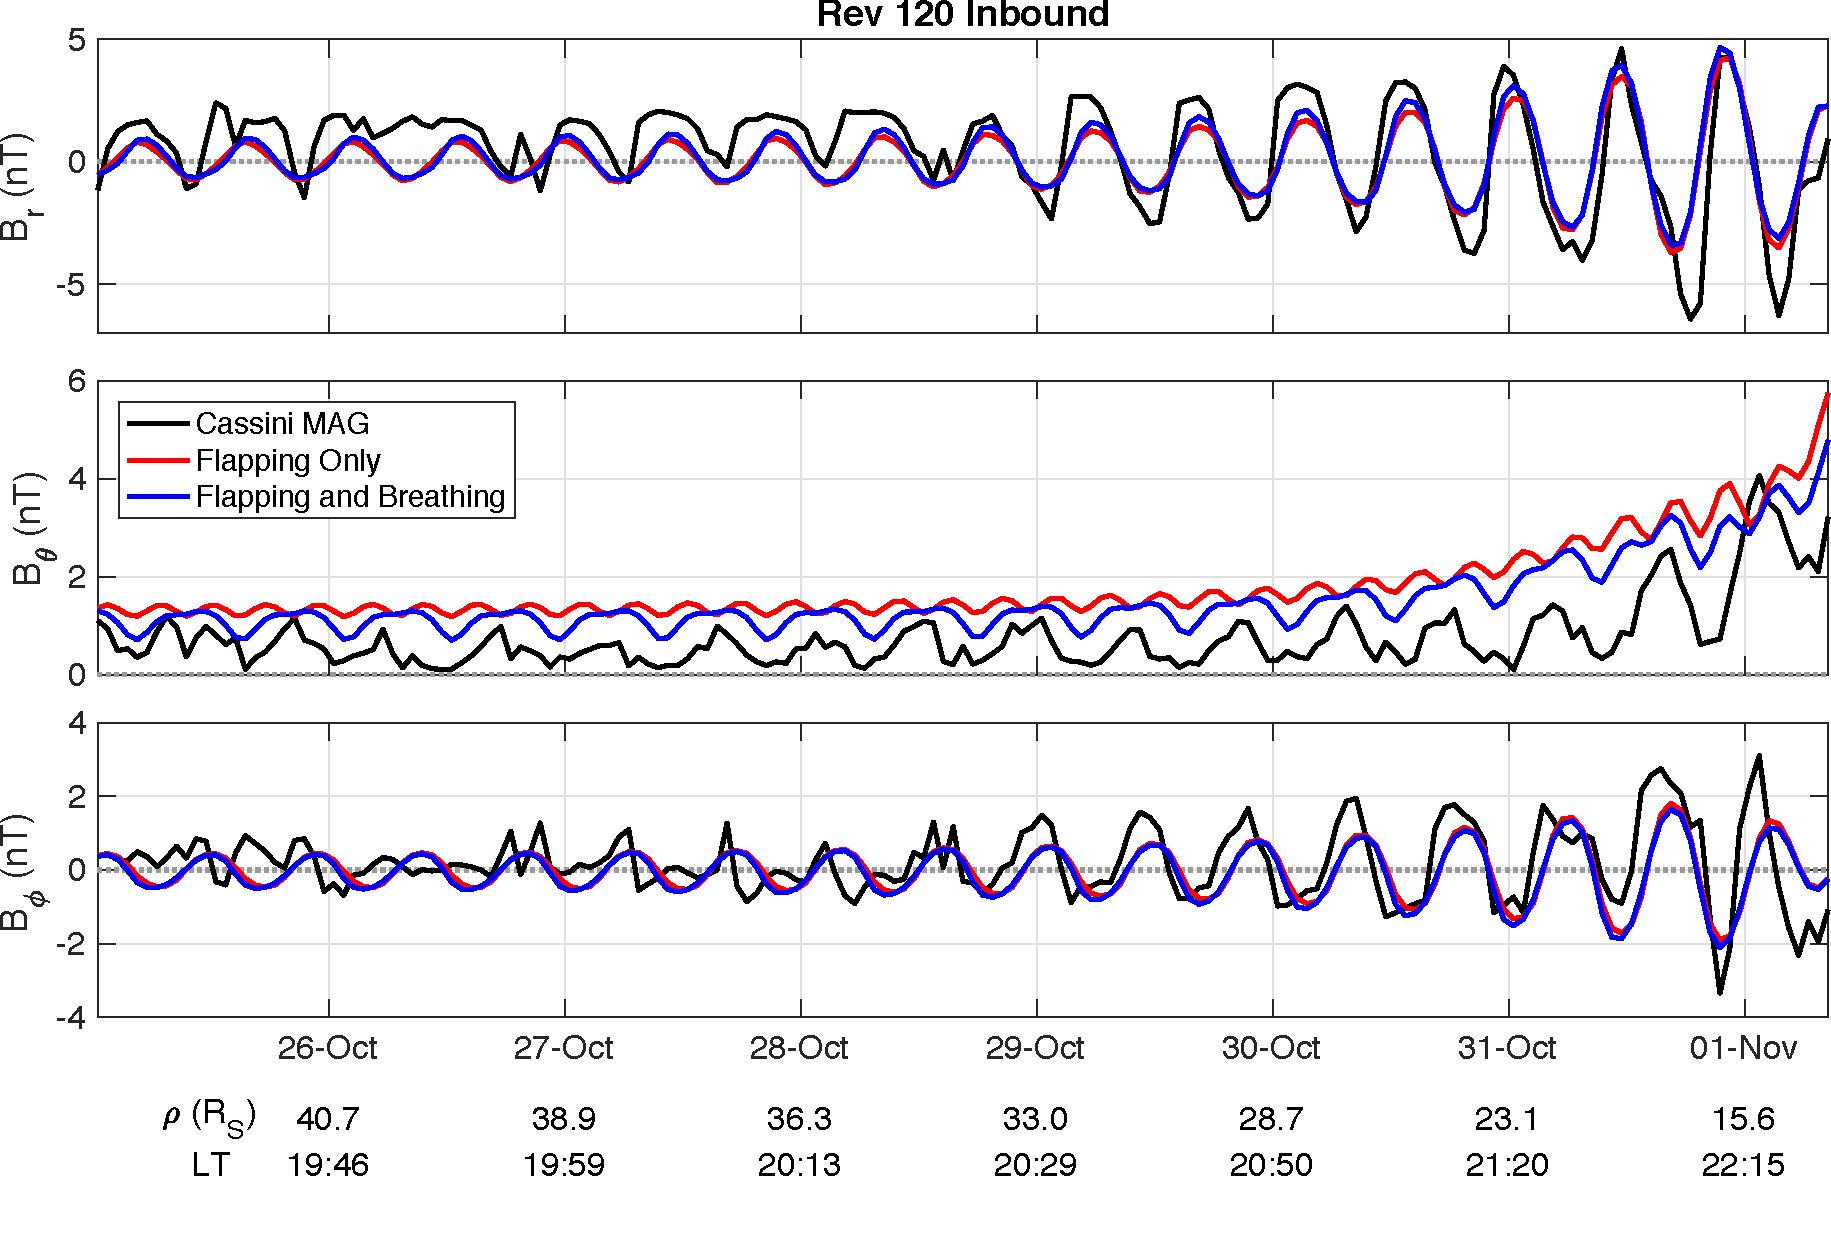
\includegraphics[width=0.9\textwidth]{equinox/rev120in.pdf}
\caption[\textit{Cassini} magnetic field data, FO and F{\&}B model predictions for Rev 120 Inbound.]{Radial (a), meridional (b) and azimuthal (c) components of the magnetic field measured by \textit{Cassini} along \textbf{Rev 120 Inbound}, outside of $\rho~{=}~\SI{12}{R_S}$ and inside the magnetosphere. In black we show the MAG data, in red is the flapping only model, and in blue is the flapping and breathing model, both with best fit parameters shown in Table~\ref{equinox:table:fitparams}. Annotation labels underneath give $\rho$, the cylindrical radial distance of \textit{Cassini} from the planet in KMSAG coordinates and the Saturn magnetic local time LT.}
\label{equinox:fig:rev120in}
\end{figure}
\begin{figure}
\centering
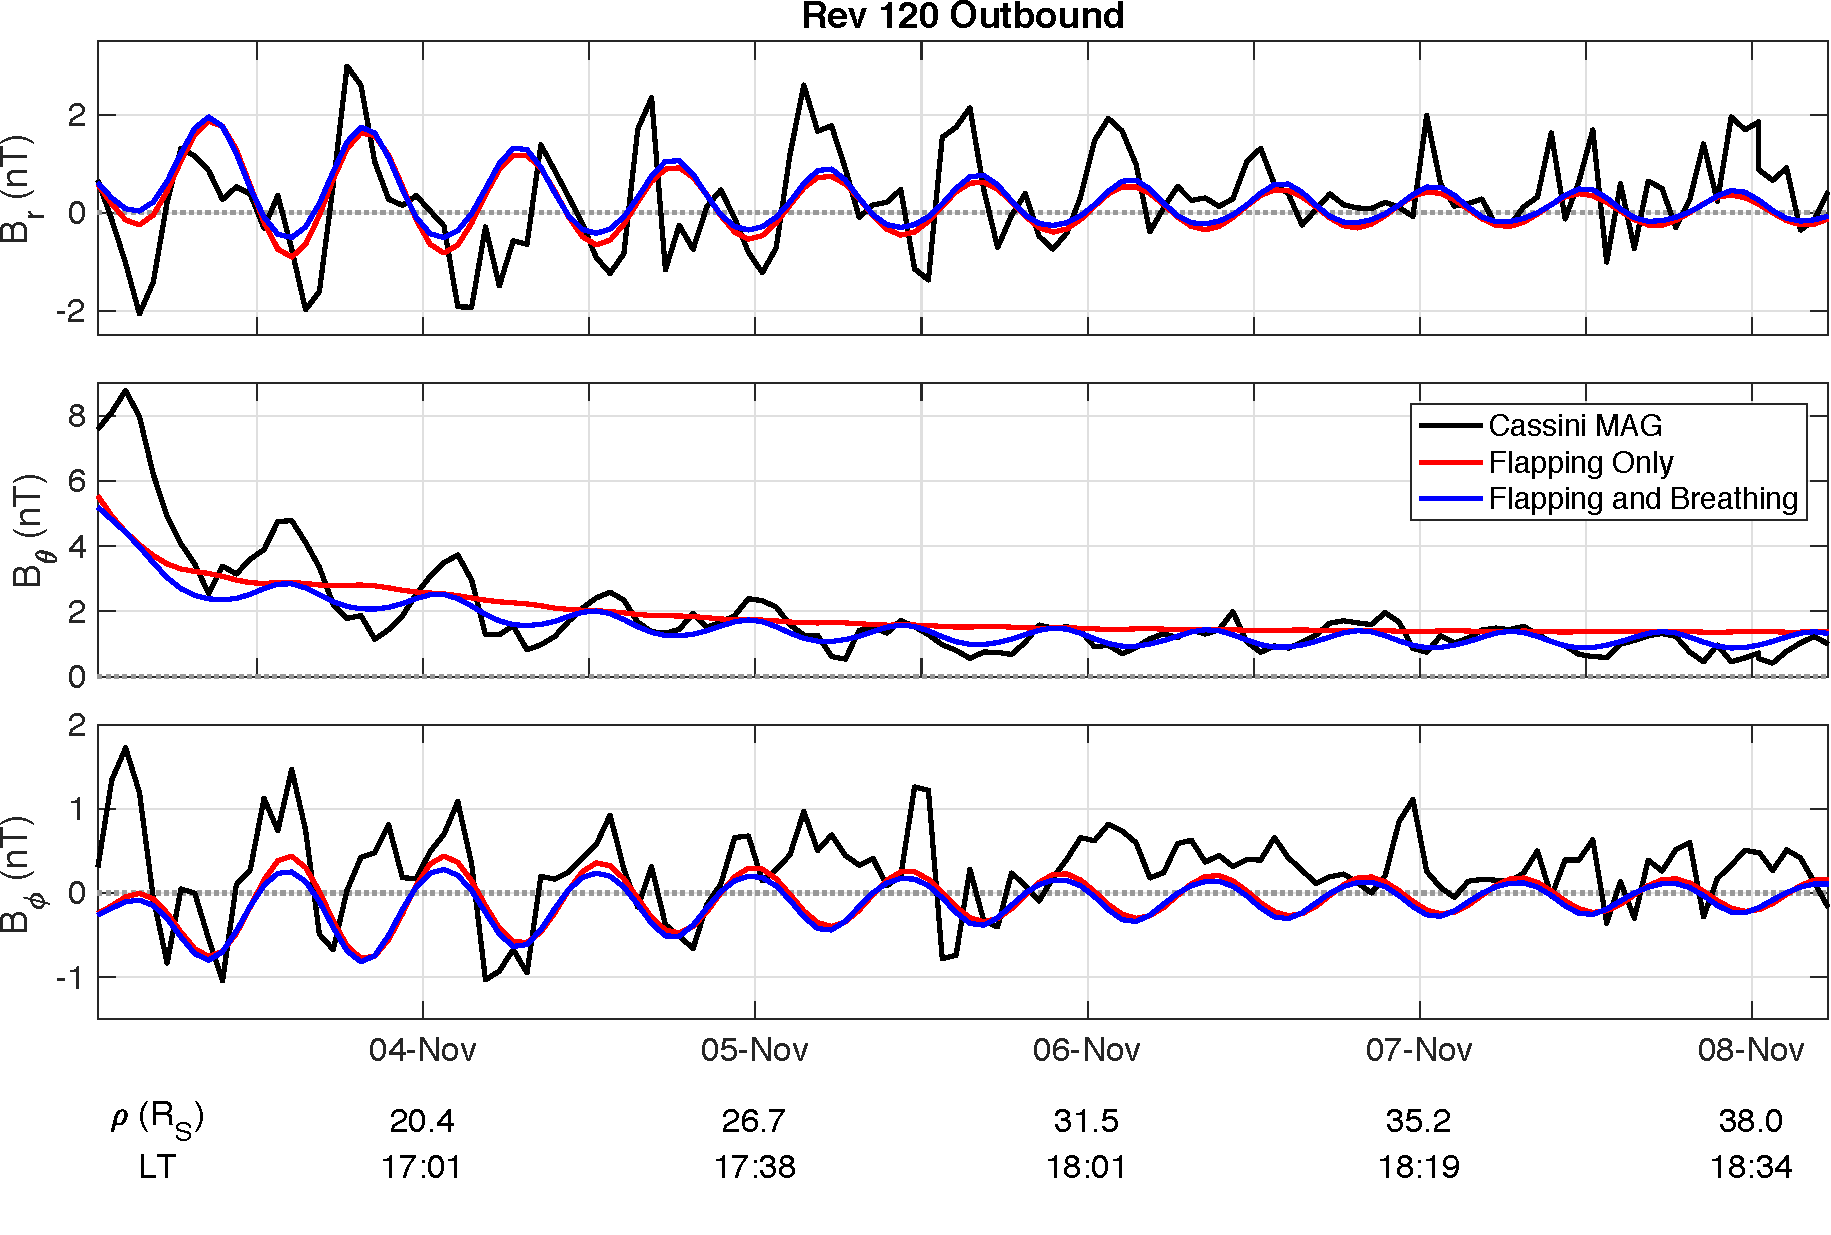
\includegraphics[width=0.9\textwidth]{equinox/rev120out.pdf}
\caption[\textit{Cassini} MAG data, FO and F{\&}B model predictions for Rev 120 Outbound.]{As for Figure~\ref{equinox:fig:rev120in} for \textbf{Rev 120 Outbound}.}
\label{equinox:fig:rev120out}
\end{figure}
\begin{figure}
\centering
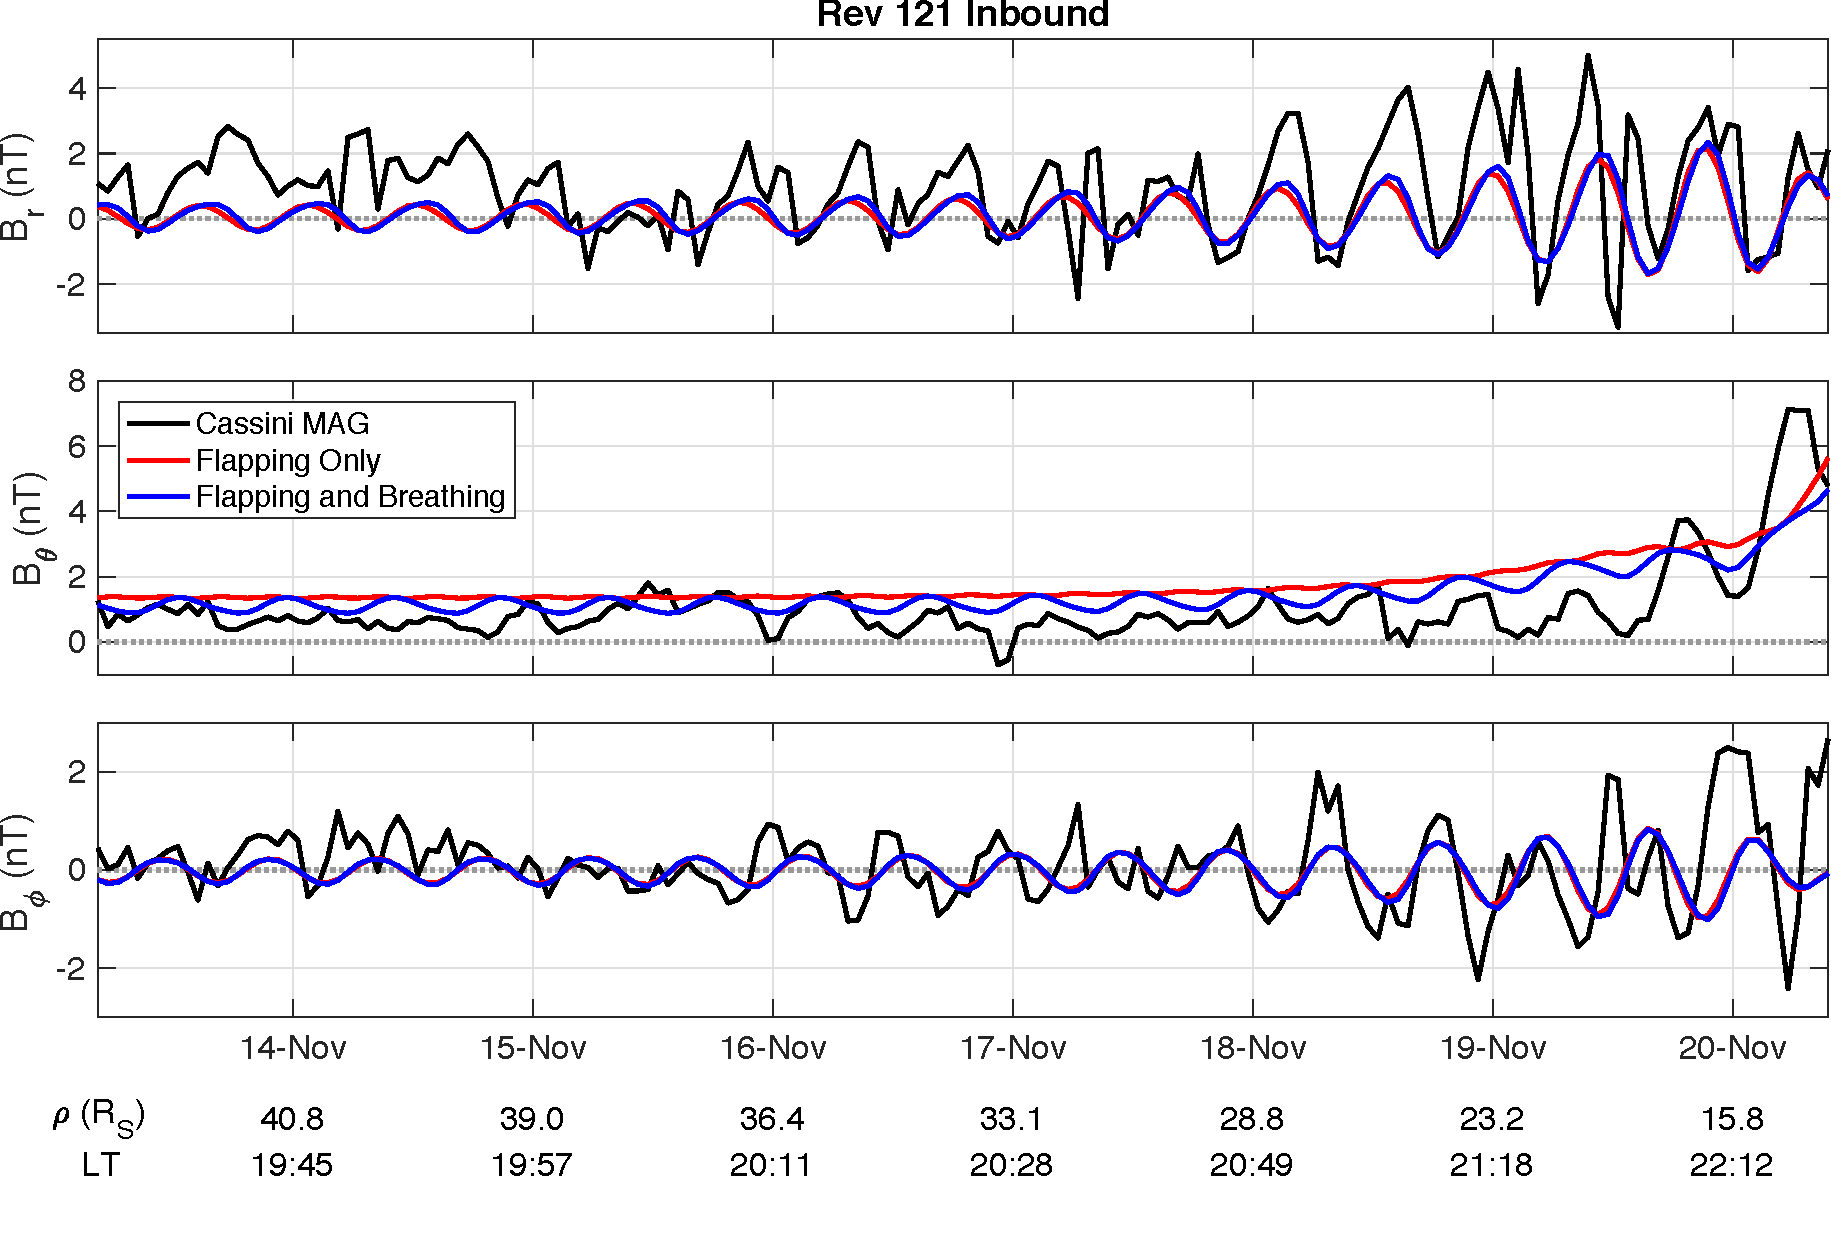
\includegraphics[width=0.9\textwidth]{equinox/rev121in.pdf}
\caption[\textit{Cassini} MAG data, FO and F{\&}B model predictions for Rev 121 Inbound.]{As for Figure~\ref{equinox:fig:rev120in} for \textbf{Rev 121 Inbound}.}
\label{equinox:fig:rev121in}
\end{figure}
\begin{figure}
\centering
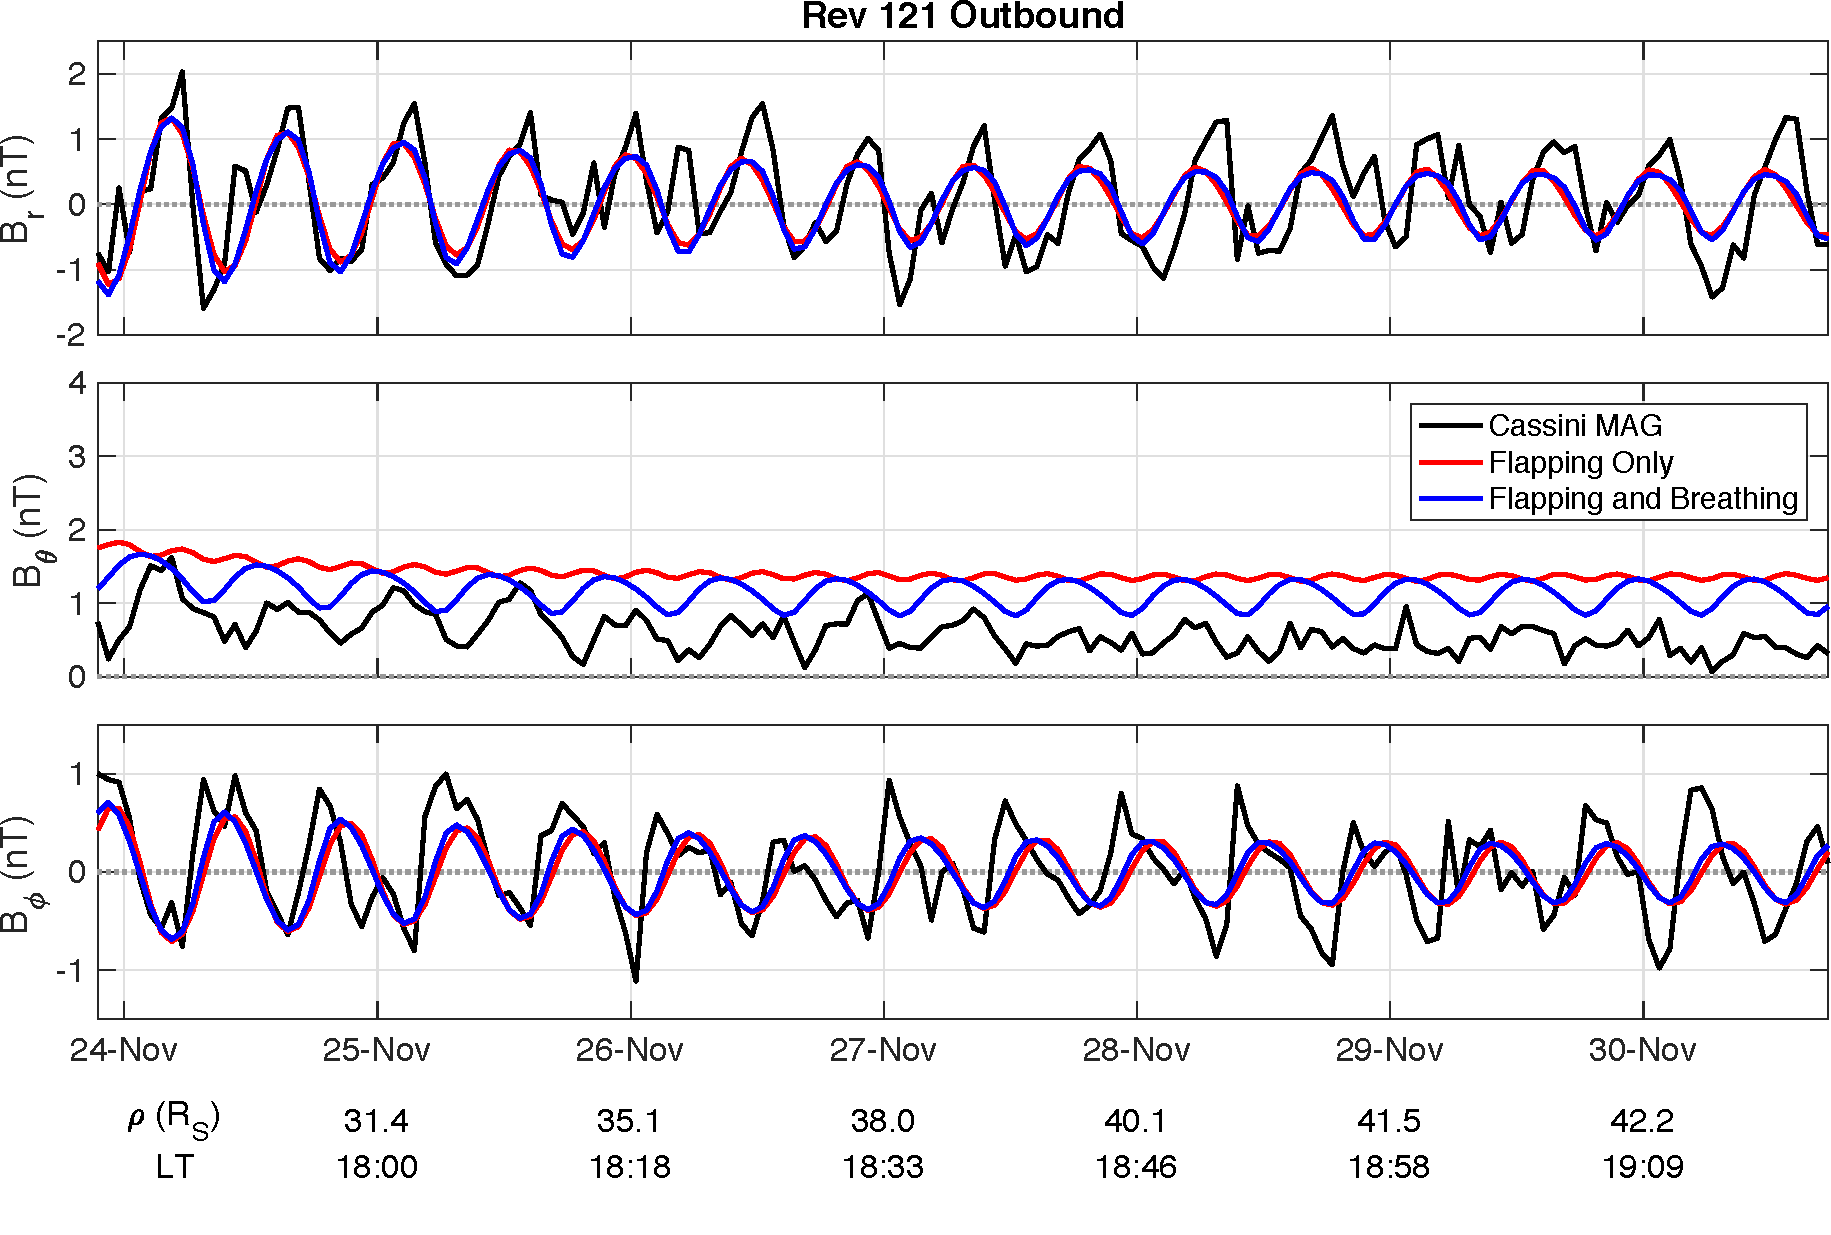
\includegraphics[width=0.9\textwidth]{equinox/rev121out.pdf}
\caption[\textit{Cassini} MAG data, FO and F{\&}B model predictions for Rev 121 Outbound.]{As for Figure~\ref{equinox:fig:rev120in} for \textbf{Rev 121 Outbound}.}
\label{equinox:fig:rev121out}
\end{figure}
\begin{figure}
\centering
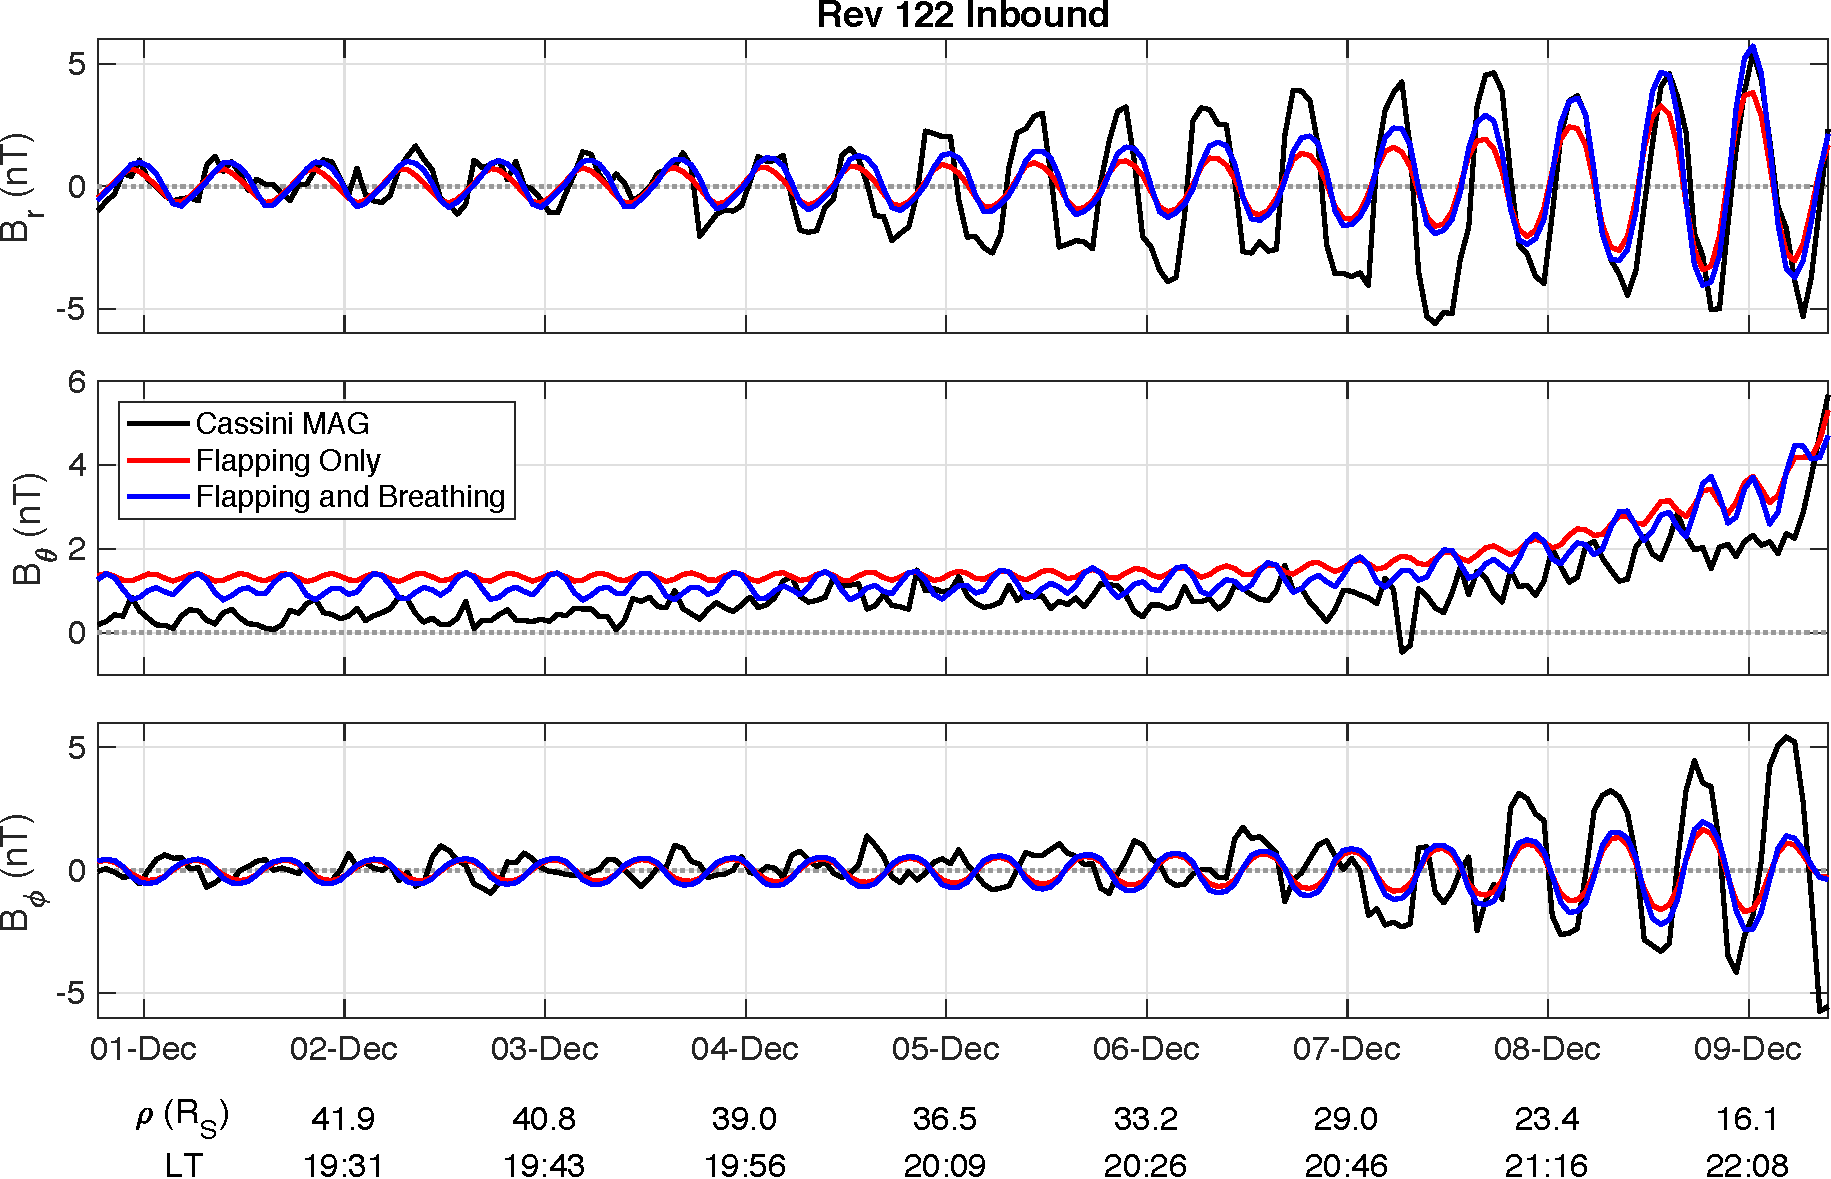
\includegraphics[width=0.9\textwidth]{equinox/rev122in.pdf}
\caption[\textit{Cassini} MAG data, FO and F{\&}B model predictions for Rev 122 Inbound.]{As for Figure~\ref{equinox:fig:rev120in} for \textbf{Rev 122 Inbound}.}
\label{equinox:fig:rev122in}
\end{figure}
\begin{figure}
\centering
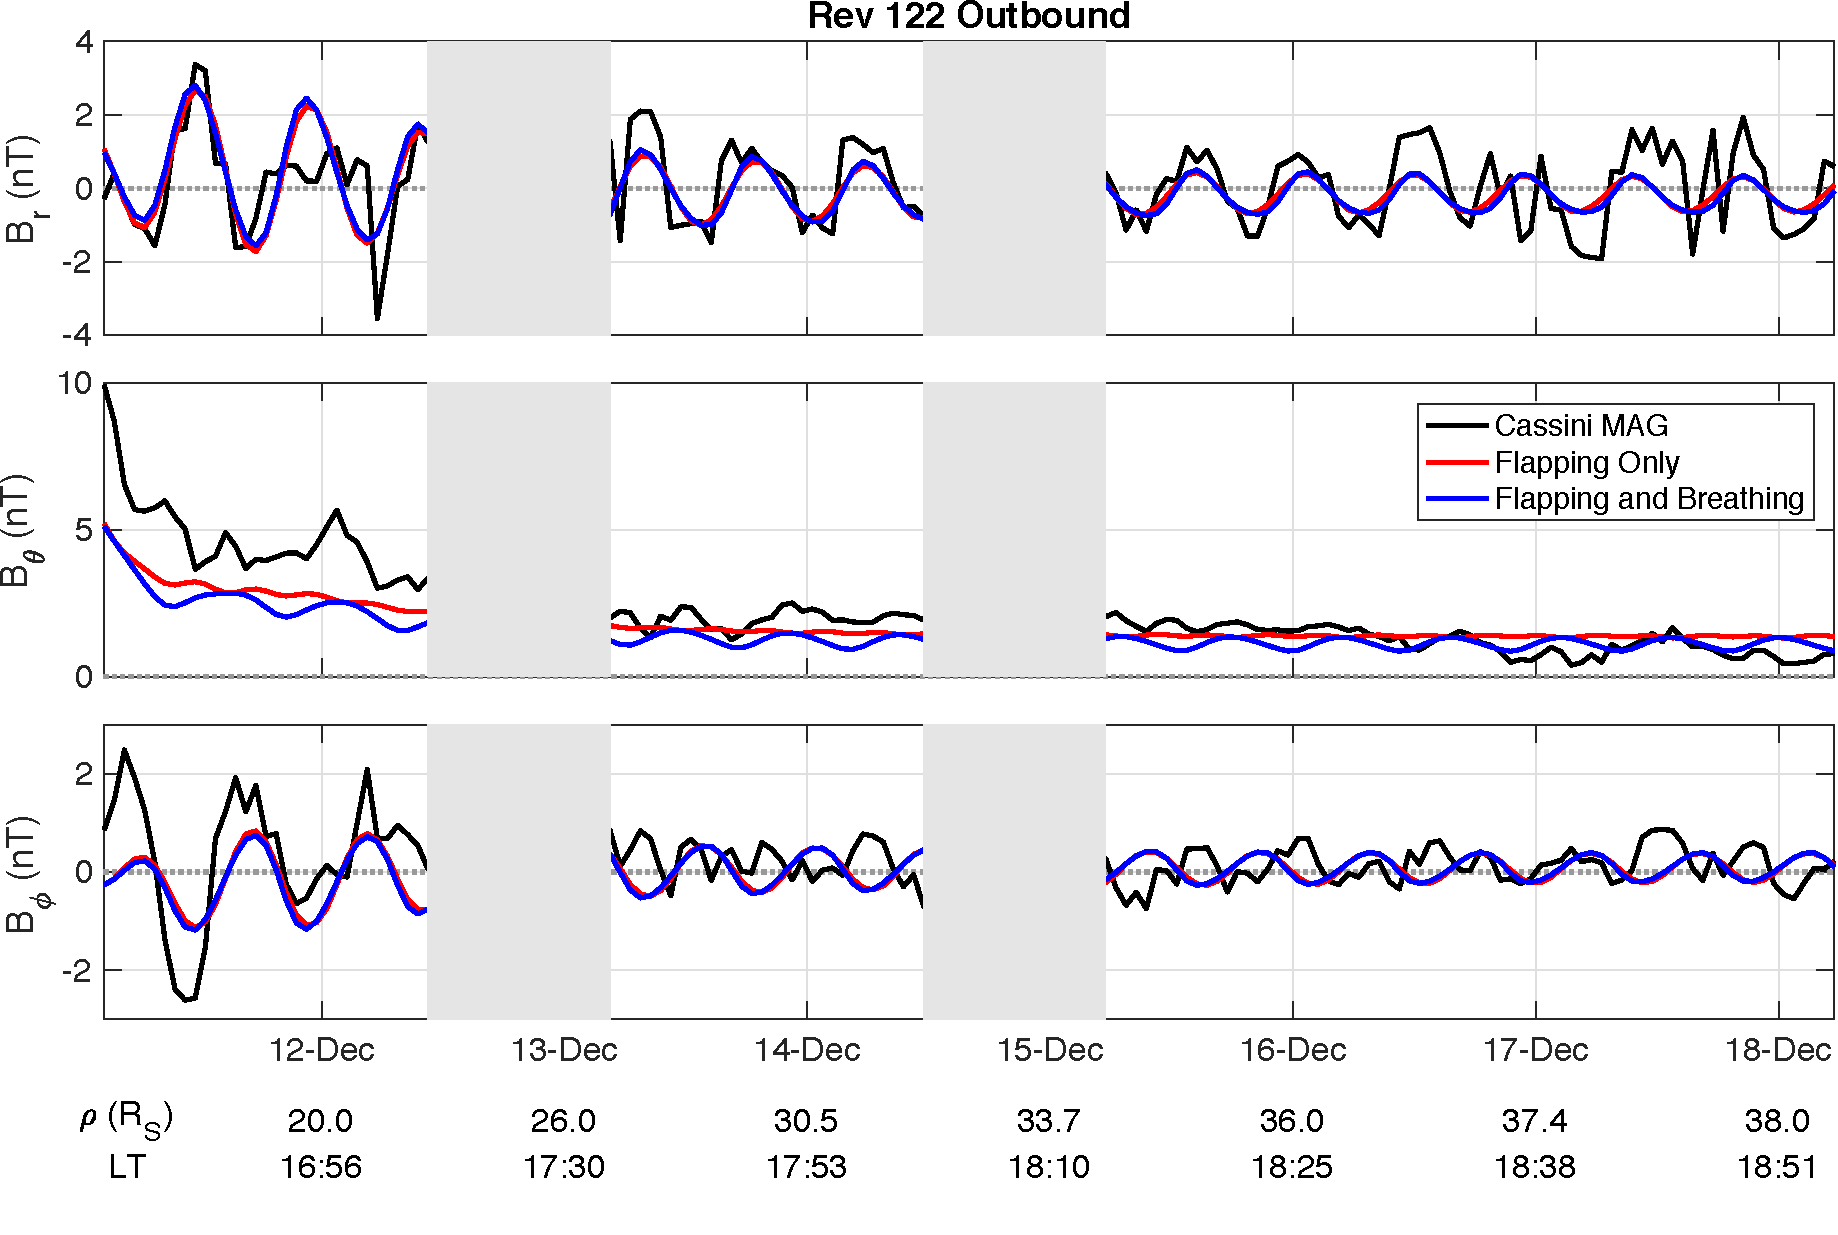
\includegraphics[width=0.9\textwidth]{equinox/rev122out.pdf}
\caption[\textit{Cassini} MAG data, FO and F{\&}B model predictions for Rev 122 Outbound.]{As for Figure~\ref{equinox:fig:rev120in} for \textbf{Rev 122 Outbound}. The grey shaded regions correspond to where \textit{Cassini} was outside of the magnetosphere and so the model was not fit to data in these regions.}
\label{equinox:fig:rev122out}
\end{figure}
Figures~\ref{equinox:fig:rev120in}~to~\ref{equinox:fig:rev122out} show the Cassini magnetic field data acquired on each pass, and the predictions by the `flapping only' and `flapping and breathing' models. The corresponding best fit parameters are shown in Table~\ref{equinox:table:fitparams}. Also shown is the root-mean-square difference (RMS) between the model and data magnetic field values for each model, equivalent to $\sqrt( \chi^2/n)$.

In general we can see that for passes that show clear periodicities in the magnetic field data, the `flapping only' (FO) model characterizes these oscillations well, particularly in the radial ($B_{r}$) and azimuthal ($B_\phi$) components. This is most clearly shown in Figures~\ref{equinox:fig:rev120in} and \ref{equinox:fig:rev121out}. For all passes, the best fit values of $\theta_\mathrm{T}$ with the FO model are in broad agreement with the literature discussed in Section~\ref{equinox:sec:intro}, although with considerable variation pass to pass. Note that the y-axis scales are not exactly the same for Figures~\ref{equinox:fig:rev120in} to \ref{equinox:fig:rev122out}, and that therefore the amplitudes of the oscillations in the magnetic field data significantly vary from pass to pass. Similarly for $\lambda_0$, with the exception of Rev 121 Inbound, our values are consistent with those of \citet{arridge2011}, who found their fits for a parameter equivalent to $\lambda_0$ varied from $101{\--}\SI{292}{\degree}$ between passes.

However we can also see that in almost all passes, the FO model does not well reproduce the oscillations in the meridional ($B_{\theta}$) component. Similar discrepancies between model and data were observed in \citet{achilleos2014}, who used a similar model construction as for the FO model discussed here. (In \citet{arridge2011} the measured meridional component of the magnetic field was not compared to the model prediction.) In particular in this study, the FO model predicts a oscillation in $B_{\theta}$ of very small amplitude compared to the observations, and with a period approximately twice that of the rotation period. This can be understood as follows: in the FO model, the only source of periodicity is the vertical displacement of the current sheet, which moves across the spacecraft twice per planetary rotation, once from above the rotational equator and once from below. In this picture the $B_{r}$ and $B_{\phi}$ components are both oppositely oriented either side of the current sheet, with $B_{r}$ maximum positive above the current sheet due to the magnetodisc magnetic field structure, and $B_{\phi}$ maximum negative above the current sheet due to the bending back of magnetic field lines, due to the lag in plasma corotation. These components are then reversed when \textit{Cassini} is under the current sheet, and therefore even for the relatively simple FO model, these magnetic field components show a full oscillation roughly once per planetary rotation, in antiphase with each other. In contrast, in the FO picture, $B_{\theta}$ varies symmetrically either side of the current sheet, with a maximum at the current sheet center and a minimum both above \textit{and} below, and hence it varies twice per planetary rotation, maintaining the same (positive) algebraic sign. For observations where \textit{Cassini's} orbit is persistently above or below the flapping current sheet, this would appear as a single oscillation in $B_{\theta}$, once per planetary rotation, with a single maximum observed when the current sheet is closest to the spacecraft. However in the trajectories being studied here, as shown in Figure~\ref{equinox:fig:cassinitrajectory}, \textit{Cassini} is orbiting extremely close to the rotational equator and thus close to the mean location of the current sheet. Therefore the current sheet flaps fully above and below the spacecraft every rotation, giving a double oscillation in the $B_{\theta}$ component.

It is for this reason that the F{\&}B model much better characterizes the $B_{\theta}$ component in these instances. This is particularly clear in Figures~\ref{equinox:fig:rev120in}, \ref{equinox:fig:rev120out}, \ref{equinox:fig:rev121in} and \ref{equinox:fig:rev121out}, where the introduction of the breathing behavior improves the characterization of both the amplitude and phase of the oscillations in $B_{\theta}$. Specifically for the phase, we now observe an oscillation in $B_{\theta}$ only approximately once per planetary rotation. In the `breathing' picture we discussed in Section~\ref{equinox:sec:intro}, this is interpreted as the `breathing in' or compression of the magnetic field lines and thickening of the current sheet at one phase of the perturbation $\lambda$, corresponding to a maximum in $B_{\theta}$, and the `breathing out' and thinning of the current sheet at the diametrically opposite phase, corresponding to a minimum in $B_{\theta}$. The phase is related to Saturn longitude as per equation~\ref{equinox:eq:lambda}, and so as the planet rotates, a stationary observer would pass through each of these longitudes once per rotation, causing a single dominant oscillation in $B_{\theta}$, as predicted by the F{\&}B model. The better agreement between this improved model and the MAG data for the passes referenced above supports the picture described in Section~\ref{equinox:sec:intro} and illustrated in Figure~\ref{equinox:fig:CowleyTDdiagrams}, that the rotating magnetic perturbations do cause a periodic modulation in the current sheet thickness as well as location. For all but Rev 122 Outbound, the F{\&}B model has a slightly lower RMS than the FO model as shown in Table~\ref{equinox:table:fitparams}, suggesting better agreement with the data, however we note that for all trajectories shown here the difference in RMS values between the FO and F\&B models is very minor.

The amplitude of the $B_{\theta}$ oscillations in the F{\&}B model is controlled by the harmonic variation in disk radius $R_\mathrm{D}=45{\--}\SI{55}{R_S}$. In some passes this amplitude appears somewhat underestimated by the model, suggesting a larger range of $R_\mathrm{D}$ and thus a larger range in current sheet thicknesses at different longitudes would be more appropriate. However we soon approach the limits of possible convergence for our magnetodisc model when using such high values of $R_\mathrm{D}$, and, as discussed in Section~\ref{equinox:sec:simulatingbreathing}, such large values for the magnetopause location would not be physically justifiable. This issue is a consequence of the model construction, as the variation in current sheet thickness in the model can only be controlled indirectly via the range in $R_\mathrm{D}$. Nevertheless, for illustration, in Figure~\ref{equinox:fig:rev121outdiffMDs} we reproduce the F{\&}B model shown in Figure~\ref{equinox:fig:rev121out}, and compare with a model using the same best fit parameters for Rev 121 Outbound, but employing a larger range of disk radii. In this illustrative model we use the original family of five magnetodisc models as described in Section~\ref{equinox:sec:simulatingbreathing}, supplemented with a larger model with $R_\mathrm{D}=\SI{65}{R_S}$, such that the total range is $\SI{20}{R_S}$. We show this comparison for Rev 121 Outbound in particular because of the approximate $\SI{90}{\degree}$ difference between the northern and southern perturbation phases, and the best-fit values for the flapping and breathing prime meridians, as shown in Table~\ref{equinox:table:fitparams}. This gives good conditions for observing the `sawtooth' signature particularly in the radial component of the magnetic field. As described in the Introduction, this signature is associated with the spacecraft traversing a thinner part of the current sheet in one part of the planetary rotation cycle, and a thicker part in the opposite part \citep{cowley2017a} and so is more prevalent when there is a more extreme variation in current sheet thickness in different hemispheres. This produces an asymmetric periodic sawtooth-like signature due to the longer time taken to traverse a thicker current sheet. 

Reassuringly, when we re-fit this new illustrative model with $\SI{20}{R_S}$ range in $R_\mathrm{D}$ to the MAG data for Rev 121 Outbound, we find that the resulting best fit parameters $\theta_\mathrm{T}$, $\lambda_0$ and $\lambda_\mathrm{B}$ are equivalent to those for our F{\&}B model for that Rev within uncertainties (although note that in Figure~\ref{equinox:fig:rev121outdiffMDs} we show the illustrative model with the exact same parameters as for our original model as shown in Table~\ref{equinox:table:fitparams}, for more direct comparison). However we can see that for the illustrative model the sawtooth signature in the radial field is indeed more pronounced, due to the more extreme range in current sheet thickness for the set of magnetodisc models used here. In addition the amplitude of oscillations in $B_{\theta}$ are greater, for the same reason. This shows the inevitable sensitivity of our results to the chosen magnetodisc model parameters.
\begin{figure}
\centering
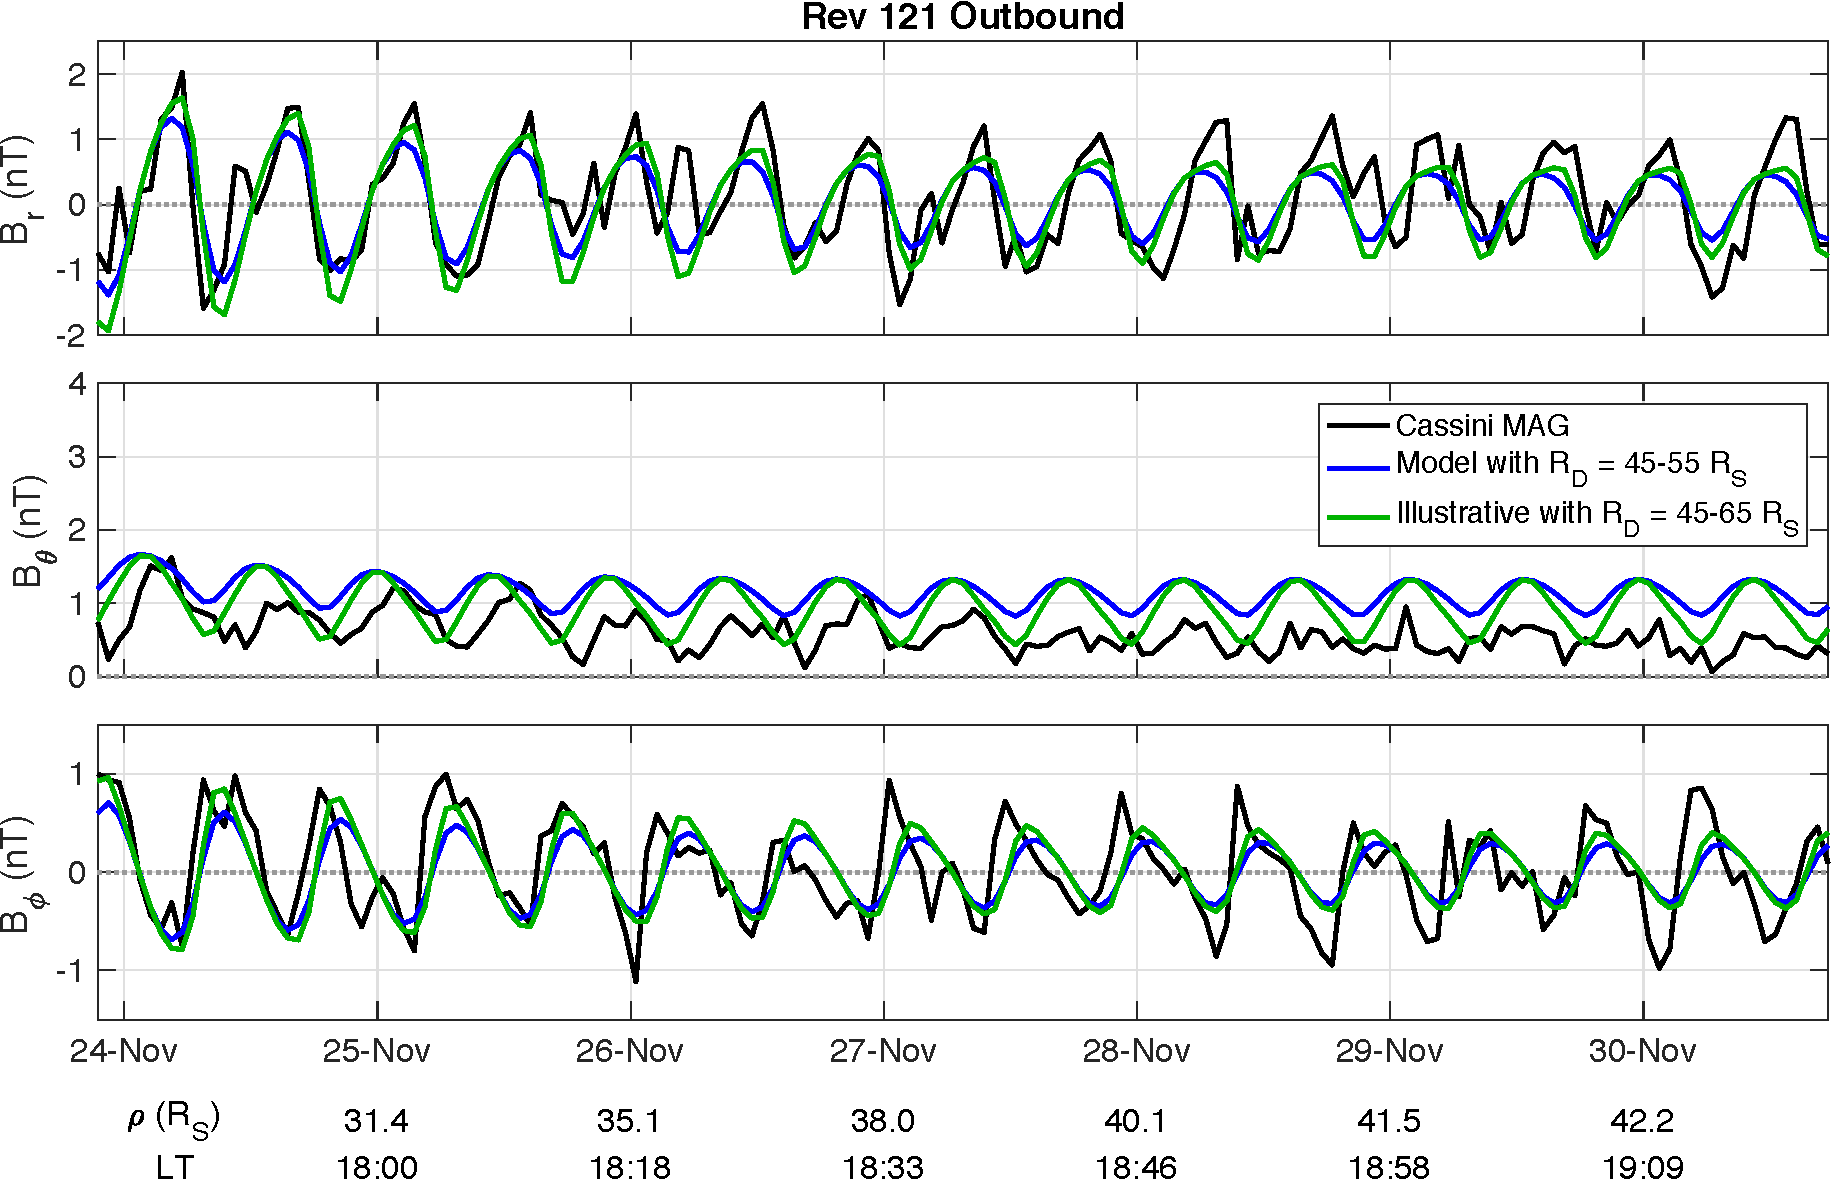
\includegraphics[width=0.8\textwidth]{equinox/rev121outdiffMDs.pdf}
\caption[\textit{Cassini} MAG data, FO and F{\&}B model predictions for Rev 121 Outbound, with modified F{\&}B model parameters.]{Similar to Figure~\ref{equinox:fig:rev120in}, for \textbf{Rev 121 Outbound}. MAG data is shown in black, in blue is a reproduction of the best-fit flapping and breathing model for Rev 121 Outbound from Figure~\ref{equinox:fig:rev121out}, and in green is flapping and breathing model using same parameters, but a larger range of magnetodisc model radii as shown by the legend.}
\label{equinox:fig:rev121outdiffMDs}
\end{figure}

The discrepancy between model and data for the average values of $B_{\theta}$ may also be due to our parameterization of the hot plasma content $K_\mathrm{H}$ in the magnetodisc model. The predicted values of $B_{\theta}$ are sensitive to our choice of $K_\mathrm{H}$, with, in general, higher hot plasma content producing higher magnetic field strengths in the outer magnetosphere, and more disk-like magnetic field structures, due to global pressure balance \citep[see][]{achilleos2010b,sorba2017}. This type of structure is also, in general, associated with a more extreme variation in the magnitude of the radial component of the magnetic field above and below the equatorial plane. Our choice of $K_\mathrm{H}$ could therefore affect our fitting of the tilt angle $\theta_\mathrm{T}$, which controls the amplitude of the oscillations in $B_r$, particularly for the FO model. As discussed in Section~\ref{equinox:sec:modelparamzation} we use a value of $K_\mathrm{H}$ appropriate for the entire data set studied here, and in line with previous results of global average values. However the appropriate $K_\mathrm{H}$ for the region local to \textit{Cassini} may well vary from pass to pass depending on local conditions, and we can see from Figure~\ref{equinox:fig:hotpressuremodel} that the hot plasma pressure varies significantly within our interval of study. This explanation would also be consistent with the observation that our models underestimate the average $B_{\theta}$ in some passes and overestimate in others, rather than systematically overestimating or underestimating across all passes. This could also potentially explain why we find a range of best-fit $\theta_\mathrm{T}$ values that, while consistent with previous results, show significant spread from pass to pass. However, we find that the observed hot plasma pressure varies significantly from a given model profile shown in Figure~\ref{equinox:fig:hotpressuremodel}, even within one single Rev as separated in this study. This comparison implies that even using different values of $K_\mathrm{H}$ from pass to pass could not capture the hot plasma variations in their entirety. Similar variability has been observed and discussed in studies such as \citet{sergis2007} and \citet{kellett2010}.

Additionally, the magnetodisc model assumption of a single ion mass along each field line, previously mentioned in Section~\ref{equinox:sec:plasmamodel}, means that the model does not account for fine variation in magnetodisc structure caused by a concentration of heavier ions near the current sheet, which could lead to a putatively thinner current sheet at large radial distance \citep{nemeth2011}. This effect would generally be associated with an even lower value of $B_{\theta}$ than we predict herein, particularly in the outer magnetosphere. Plasma sheet thickness can also vary unsystematically on timescales as short as a single \textit{Cassini orbit}, potentially due to a combination of internal and external influences, as shown by \citet{sergis2011}.

Saturn's current sheet thickness also varies with local time, which is not directly accounted for by our model, as discussed in Section~\ref{equinox:sec:simulatingbreathing}. The range in local time for each \textit{Cassini} pass studied here is only $\sim2-3.5$ hours, and so within a given pass any variation in sheet thickness associated with local time is likely to be less significant than the variation due to the magnetodisc breathing behavior. For the entire data set studied here, the local time range is approximately 15:45-22:45, with 80\% of the data in the range 18:00-21:00, which could introduce variations between passes in how well our model characterizes the data; however, observation of Figures~\ref{equinox:fig:rev120in}-\ref{equinox:fig:rev122out} does not reveal a significant relationship between model-data discrepancies and the local time range of the given pass.

Looking at each pass individually, the best fit parameters for the F{\&}B model are in general consistent with those of the FO model, suggesting that the FO model is an appropriate approximation at least for modeling the $B_{r}$ and $B_{\phi}$ components of the magnetic field. Specifically, for all but Rev 122 Inbound, the fitted values of $\lambda_0$ agree for each model within uncertainties, and the fitted values for $\theta_\mathrm{T}$ are lower for the F{\&}B model than the FO model. This can be understood as $\theta_\mathrm{T}$ controls the amplitude of the oscillations in the magnetic field associated with the flapping, and so introduction of the breathing behavior allows some of this amplitude to be `accounted for' by the breathing perturbation. It is perhaps not surprising that Rev 122 Inbound is the exception to this observed behavior, as Figure~\ref{equinox:fig:rev122in} shows there is very little observed periodic oscillation in $B_{\theta}$ during this pass, meaning the F{\&}B model is not well constrained. In addition, on this pass a transient negative $B_{\theta}$ signature can be seen around 7 December, which is associated with a region of higher density, lower energy plasma in the CAPS-ELS data. This may be a signature of a small-scale `ballooning' instability of the plasma sheet, resulting in a northward turning of the magnetic field in the center of a localized plasma `bubble', similar to events observed at Jupiter by {\citet{kivelson2005}. This event appears to perhaps be immediately preceded by an episode of current sheet thinning, as revealed by larger amplitude oscillations in the radial component of the field compared to both the model predictions, shown in Figure~\ref{equinox:fig:rev122in}.} This suggests a very dynamic plasma sheet in this region, and perhaps explains why our models do not reproduce the data for Rev 122 Inbound in particular. It is interesting to note that immediately after the event $B_\theta$ appears to peak when $B_r$ is close to 0, perhaps suggesting a return to flapping-only-like behavior after this event. Similar transient negative $B_\theta$ signatures can be seen in Rev 121 Inbound around 17{\--}18 November, (Figure~\ref{equinox:fig:rev121in}), and again are accompanied by more variable, aperiodic magnetic field signatures that cannot be characterized by our models.

In general the best fit values of $\lambda_\mathrm{B}$ show large variation pass to pass, and have larger uncertainties as they are only significantly constrained by the behavior of the $B_{\theta}$ component. As described in Section~\ref{equinox:sec:simulatingbreathing}, this parameter $\lambda_\mathrm{B}$ determines the approximate longitude at which the maximum disk model radius is used at $\rho = \rho_0$, which in our model is the same as the region with the thinnest, most radially distended current sheet. Looking at Figure~\ref{equinox:fig:CowleyTDdiagrams}, we can see that for a magnetosphere system dominated by the southern perturbation, we would expect values of $\lambda_\mathrm{B}$ and $\lambda_\mathrm{0}$ to be similar, as the maximum vertical displacement of the current sheet and the maximum radial distortion of the current sheet are at the same longitude in panel (d). While we do observe this for one pass, there is considerable spread among the other passes. Meanwhile for a system dominated by the northern perturbation, from Figure~\ref{equinox:fig:CowleyTDdiagrams} we would expect to observe $\lambda_\mathrm{B}$ and $\lambda_\mathrm{0}$ approximately $\SI{180}{\degree}$ apart, as in panel (b) the longitude of the maximum vertical displacement of the current sheet is diametrically opposite to the longitude where the current sheet is most radially distended. However we find that our measured values of $\lambda_\mathrm{B}$ are not, in general, compatible with this picture either. This suggests that the northern and southern magnetic perturbations are of similar amplitude during this time period, which indeed was observed by \citet{andrews2012}, and thus are both controlling the dynamics of the magnetodisc to varying degrees. Indeed, as described in the recent study by \citet{cowley2017b}, the true behavior of the magnetodisc is more complicated than this simplified interpretation of diagrams of Figure~\ref{equinox:fig:CowleyTDdiagrams}, with the current sheet thickness modulated differently in the northern and southern hemispheres depending on the phase difference between the two rotating magnetic perturbations. In this study we only explicitly allow one thickness modulation, at the phase $\lambda = \lambda_\mathrm{B}$, and so even our F{\&}B model cannot fully resolve this behavior. In a study by \citep{provan2012}, the authors observe that the modulation in current sheet thickness is most extreme, by a factor of ${\sim}2$, when the northern and southern perturbations are in antiphase. In this study we use a fixed current sheet thickness modulation, fully controlled by our chosen range in disk model radius $R_\mathrm{D}$, and so cannot resolve at what phase differences we observe the greatest variation in current sheet thickness. However we intend to address this in a future study either by allowing the range of $R_\mathrm{D}$ to vary as a free parameter, or similar alternative approaches, discussed below in Section~\ref{equinox:sec:constDp}.

Another complicating factor for our best fit parameters is our choice of the delay parameter $D = \Omega_S/v_\mathrm{w} = \SI{3}{\degree/R_S}$. This predominantly influences the phasing rather than the amplitude of the model oscillations; for larger values of $D$, the spiral pattern shown in Figure~\ref{equinox:fig:cssurfacemodel} becomes more tightly wound, and so the period of the oscillations generally becomes shorter with increasing radial distance. This particularly affects our fitting of the parameter $\lambda_0$, as this parameter also influences the model phasing by controlling the phase of the maximum flapping perturbation. As previously discussed, the data sets studied here are restricted in local time to the dusk sector, with the majority of observations in the local time sector 18:00{\--}21:00, and no single pass spanning more than 3.5 hours of local time. Therefore the aforementioned variation in magnetospheric wavespeeds reported in \citet{andrews2010} is unlikely to have a large influence. However the possible variation in wavespeeds with radial distance and local conditions, as discussed in Section~\ref{equinox:sec:cssmodel}, may be a source of discrepancy between our models and results. 

As a preliminary investigation, we re-fit the F{\&}B model to the Rev 120 Inbound pass data using a greater value for the delay parameter $D = \SI{5}{\degree/R_S}$, chosen as roughly the upper limit of an expected appropriate value for $D$ as discussed in Section~\ref{equinox:sec:cssmodel}. We found that the resulting best fit parameters were not significantly altered for this fit, with $\theta_\mathrm{T}$ and $\lambda_\mathrm{B}$ both equivalent to the values presented in Table~\ref{equinox:table:fitparams} within uncertainties, and the value of $\lambda_0$ differing by around 9\%, broadly as expected as this parameter is most strongly affected by the phasing controlled by the specific value of $D$. We also found that the RMS residual between model and data was around 6\% greater for this model than for our original model with $D = \SI{3}{\degree/R_S}$, suggesting this original lower value of $D$ is appropriate for the best fit in this case.

In addition, with the F{\&}B model we attempt to characterize both the rotational flapping perturbation and the compressional breathing perturbation. Intuitively, the delay in the flapping perturbation could be considered to be controlled by the local Alfv\'{e}n speed of the magnetospheric plasma, with information traveling from the magnetic poles to the current sheet along magnetic field lines, because this is a rotational perturbation causing a displacement of the current sheet. In contrast the breathing perturbation could be considered to be controlled by the plasma magnetosonic speed, with information traveling radially outwards in the equatorial region towards the outer magnetosphere, perpendicular to magnetic field lines, because this is a compressional perturbation. This means that it may be more appropriate to use different delay parameters for the two different perturbations. This more complicated picture for local phase determination is beyond the scope of this current work, but would be rewarding to investigate in future.

As discussed in Section~\ref{equinox:sec:method}, in this study we use a longitude system based on the southern magnetic perturbation from \citet{andrews2012}, as the amplitude of this perturbation was greater than or similar to the northern perturbation in the equinox period being studied here. In addition, this allowed for a direct comparison with the results of \citet{arridge2011}. However there is no fundamental physical reason why we could not have used a system based on the northern magnetic perturbation instead. While the amplitude of the oscillations in the magnetic field are unlikely to be affected by such a change, the phasing of the oscillations would be, as the rotation period associated with the northern perturbation is shorter than for the southern. However, as discussed in Section~\ref{equinox:sec:intro}, this difference became smaller in the period after Saturn equinox, to around $\SI{0.1}{\hour}$ for the time period being studied here. A preliminary investigation with the Rev 120 Inbound pass showed that the best fit parameters were not significantly altered when using the northern perturbation to organize the oscillations, with the best fit $\theta_\mathrm{T}$ equivalent to the value presented in Table~\ref{equinox:table:fitparams} within the measured uncertainty, and the difference between the parameters $\lambda_0$ and $\lambda_\mathrm{B}$ for the F{\&}B model also the same within uncertainties to the results presented here. Note that when using the northern perturbation we would not expect the actual absolute values for $\lambda_0$ and $\lambda_\mathrm{B}$ to be equal to those presented here, as they would be measured relative to that new longitude system. Therefore only the difference between the two parameters is comparable, and even this value is somewhat influenced by using the new longitude system due to the aforementioned difference in rotation period for the northern perturbation. Whilst by no means a comprehensive analysis, this result is reassuring and suggests that our main conclusions would not be significantly altered if we were to use the northern perturbation as a longitude system instead.


\subsection{Consideration of Equilibrium and Constant Solar Wind Dynamic Pressure}\label{equinox:sec:constDp}

If the compressional breathing perturbation, and consequent movement of the magnetopause boundary, is triggered by an internal source within the magnetosphere, then the appropriate family of magnetodisc models used to simulate this behavior should ideally represent an equivalent system under constant solar wind dynamic pressure. However in this study, the magnetodisc models contain no source of internal pressure perturbation, but are calculated assuming magnetostatic equilibrium for different disk radii, and, therefore, different upstream solar wind dynamic pressure. This is done to try and reproduce the reconfiguration in magnetic field associated with the breathing dynamics. In \citet{sorba2017}, the authors estimated the incident solar wind dynamic pressure $D_\mathrm{P}$ corresponding to a given magnetodisc model by simply summing the magnetic and plasma pressure components just inside the magnetopause boundary at the nose of the magnetodisc (the subsolar point), thus assuming pressure balance across the magnetopause. Below we attempt to use the same approach here for our family of magnetodisc models used to simulate the breathing behavior. However unlike in \citet{sorba2017}, our analysis is not restricted to the nose of the magnetodisc, where the solar wind is normal to the magnetopause surface, and we therefore must account for the angle $\psi$ between the incident solar wind and the magnetopause surface normal. In the magnetopause surface model by \citet{pilkington2015}, the authors used the relationship initially proposed by \citet{kanani2010} to estimate the incident solar wind dynamic pressure from measurements just inside the magnetosphere,
\begin{equation}\label{equinox:eq:pbalance}
\frac{B_\mathrm{MS}^2}{2\mu_0} + P_\mathrm{MS} = [k\cos^2(\psi) + \frac{k_\mathrm{B}T_\mathrm{SW}}{1.16m_\mathrm{p}u_\mathrm{SW}^2}\sin^2(\psi)] D_\mathrm{P}
\end{equation}
itself based on the formulation by \citet{petrinec1997}. The terms on the left represent the magnetospheric (hence MS subscript) magnetic and plasma pressures just inside the magnetopause boundary, and the terms on the right (the coefficients of solar wind dynamic pressure $D_\mathrm{P}$) represent the component of solar wind dynamic pressure incident on the magnetopause surface, and a smaller component associated with the solar wind's thermal pressure (see \citet{kanani2010}). $k = 0.881$ is a factor to account for the diversion of flow around the magnetosphere obstacle \citep[see][]{spreiter1966}, and $T_\mathrm{SW}$ and $u_\mathrm{SW}$ are the temperature and speed of the solar wind. It was shown by \citet{kanani2010} that the estimated dynamic pressure is insensitive to the choice of $T_\mathrm{SW}$ and $u_\mathrm{SW}$ as for any reasonable choice, this term is significantly smaller than the first $D_\mathrm{P}$ term for the full range of $\psi$ over which the magnetopause surface model is valid. Nevertheless we use the full form of equation~\ref{equinox:eq:pbalance} here with $k_\mathrm{B}T_\mathrm{SW} = \SI{100}{eV}$ and $u_\mathrm{SW} = \SI{460}{\km\per\second}$ following \citet{pilkington2015}. At the magnetopause nose $\psi = \SI{0}{\degree}$ as the magnetopause surface is perpendicular to the incident solar wind, and as you move anti-sunward along the magnetopause surface this value increases, theoretically approaching $\SI{90}{\degree}$, and so the second $D_\mathrm{P}$ term becomes comparatively greater. At the dusk flank, at the location of the most anti-sunward magnetopause crossing in our data set, shown in Figure~\ref{equinox:fig:crossingssurface}, the surface models shown there have $\psi \approx \SI{67}{\degree}$. This gives a coefficient of $D_\mathrm{P}$ in equation~\ref{equinox:eq:pbalance} of $0.135 + 0.033 \approx 0.17$. If we take our magnetodisc model family to be representative of the magnetosphere in that region, we can then estimate the incident solar wind dynamic pressure $D_\mathrm{P}$ by the sum of the internal magnetic and plasma pressures just inside the model magnetopause boundary, divided by this value 0.17, following equation~\ref{equinox:eq:pbalance}.

Table~\ref{equinox:table:EdgePs} shows this calculation for the family of five magnetodisc models that were used to simulate the breathing behavior in this study. We can see that the total pressure at the equator just inside the magnetopause boundary ($P_\mathrm{EDGE}$), and the corresponding estimate of $D_\mathrm{P}$, is not constant across all models, but is lowest for the largest magnetodisc model and varies by around 60\%. Hence, as we indicated earlier, this family of models does not represent a system under constant solar wind dynamic pressure.

For a more physically realistic model, we would ideally be able to simulate the breathing behavior of the current sheet without the need to modify the implied external solar wind dynamic pressure. One potential alternative approach, which would satisfy this particular condition, is as follows. A single magnetodisc model could be used at all longitudes, with a given disk radius $R_\mathrm{D}$, as for the flapping only model. The breathing behavior could then be simulated by varying the cylindrical radial distance $\rho_\mu$ at which magnetic field values are extracted from the magnetodisc model (see equation~\ref{equinox:eq:coordinatetransform} and discussion). This could be varied harmonically with longitude broadly as $R_\mathrm{D}$ is in our current approach, such that the local magnetodisc structure is effectively displaced inwards or outwards with respect to the spacecraft location, depending on the spacecraft longitude, while the effective solar wind dynamic pressure corresponding to that underlying magnetodisc model remains constant. While beyond the scope of the current study, this approach may provide an interesting comparison to the work presented here in terms of the amplitude and shape of the magnetic field oscillations, and may be investigated in more detail in future. The potential drawback of this approach is that it would not reveal explicitly how a periodic thickening and thinning of the current sheet affects the magnetic field oscillation signatures, but more how the global magnetodisc magnetic field structure varies with radial distance. While it satisfies the condition that the incident solar wind pressure is not modulated, it is a somewhat artificial method of introducing the breathing behavior and is thus a low-order approximation of the true behavior of the magnetodisc. Alternatively, a longitude-dependent scaling factor representing sheet thickness could be used to multiply the model coordinate $z_\mu$ (see equation~\ref{equinox:eq:coordinatetransform}. The longitude dependence could be controlled by a free parameter (much as $\lambda_\mathrm{B}$ is used in this study), but we could also potentially fit for the value of the scale factor; in this way we could investigate by how much the current sheet thickness varies for different phase differences between the Northern and Southern magnetic perturbations, and thus compare results more directly with the observations of \citep{provan2012} and \citep{cowley2017b}.
\begin{table}
\caption[Model radii and solar wind dynamic pressure estimates for breathing magnetodisc models.]{Table showing the 5 different magnetodisc models used in this study to simulate the breathing behavior, their disk radii $R_\mathrm{D}$, the total magnetic and plasma pressure at the equator just inside the magnetopause boundary $P_\mathrm{EDGE}$, and the corresponding estimate of solar wind dynamic pressure $D_\mathrm{P}$ using equation~\ref{equinox:eq:pbalance}.}
\label{equinox:table:EdgePs}
\centering
\begin{tabular}{c c c}
\hline
$R_\mathrm{D}~(\si{R_S})$ & $P_\mathrm{EDGE}~(\si{nPa})$  & Approx $D_\mathrm{P}~(\si{nPa})$\\
\hline
45 & 0.0027 & 0.016 \\
47.5 & 0.0023 & 0.014\\
50 & 0.0020 & 0.012 \\
52.5 & 0.0018 & 0.011 \\
55 & 0.0016 & 0.010 \\
\hline
\end{tabular}
\end{table}

\section{Summary and Conclusions}\label{equinox:sec:conclusions}
In this study, we have investigated the periodic dynamical behavior of Saturn's equatorial current sheet during the period following Saturn equinox in late 2009, using data from \textit{Cassini's} magnetometer instrument. We have attempted to model both the periodic vertical displacement of the current sheet above and below the rotational equator (`flapping' behavior) and the periodic thickening and thinning of the equatorial current sheet, and corresponding change in magnetic field structure from more dipolar to more disk-like (`breathing' behavior). Both of these behaviors are thought to be controlled by the dual rotating magnetic perturbations that have been observed in Saturn's northern and southern hemispheres.

To do this modeling we have used a local, force-balance magnetic field and plasma model of Saturn's magnetodisc from \citet{achilleos2010a}, and geometrically anchored it to a global, geometric model of current sheet location from \citet{arridge2011}. The flapping behavior is simulated by the periodic displacement of the model current sheet location, and the breathing behavior is simulated by varying the magnetodisc model disk radius, and thus the magnetic field structure, with azimuth around the planet.

We find that, for those passes that show clear periodic oscillations in the magnetic field, our model characterizes well both the amplitude and phase of the oscillations. In particular, the $B_\theta$ (meridional) component of the magnetic field is in general better characterized when the breathing behavior is included, as it can better replicate both the amplitude and the dominant variation once per rotation period, rather than twice as with the flapping only model. These observations therefore support the picture described in Section~\ref{equinox:sec:intro} and previously observed by studies described therein, that the dual rotating magnetic perturbations in Saturn's magnetosphere cause a periodic modulation in the current sheet thickness, as well as in location above or below the rotational equator. In particular, we find that the \citet{arridge2011} tilted, rippled current sheet model with a value of delay parameter $D = \SI{3}{\degree/R_S}$ can accurately characterize the periodic flapping behavior of the magnetodisc, with observed tilt angles $\theta_\mathrm{T}$ in the range $4-\SI{18}{\degree}$ for the trajectories studied here, in line with previous studies discussed in Section~\ref{equinox:sec:intro}. We also find values of $\lambda_0$ that, when using the Southern magnetic perturbation from \citet{andrews2012}, are broadly consistent with the results of \citet{arridge2011}. For the breathing parameter introduced in this study, $\lambda_\mathrm{B}$, we find a wide variation between \textit{Cassini }passes, suggesting that this behavior varies significantly on this timescale relative to the prime meridian of the flapping perturbation, likely due to the changing strengths and phase differences between the Northern and Southern magnetic perturbations. However we have shown that by harmonically varying the model disk radius by $\SI{10}{R_S}$, from $45-\SI{55}{R_S}$, we can semi-quantitatively reproduce the oscillations in the magnetic field components associated with a periodic perturbation in current sheet thickness, as described in previous studies discussed in Section~\ref{equinox:sec:intro}. This suggests that the variation in current sheet thickness between these different-sized magnetodisc models, shown in Figure~\ref{equinox:fig:MDALLcsthickness}, is broadly representative of the magnetodisc behavior for the time interval studied.

For some passes the observed magnetic field is very variable on short timescales, perhaps due to local transient events in Saturn's plasma sheet, and our model is not capable of capturing this dynamical behavior. In addition, one main drawback of our model is that it does not explicitly take into account the phase difference between the northern and southern rotating magnetic perturbations, instead using the phase of the southern magnetic perturbation in particular to organize the magnetic field data. This limits the the physical insights we can draw from our observations, and we intend to develop this aspect of the model further in a future study. However, the relative strength of the current approach is that the model can capture the observed behavior of the magnetic field rather well for much of the time interval studied, with relatively few fitted or fixed parameters.

The treatment of the delay parameter $D$, discussed in Section~\ref{equinox:sec:method}, is another area where we intend to develop this model further, perhaps using other data sets to further constrain the appropriate choice of $D$, and in particular how it may vary with radial distance and local time. This may improve the agreement between the model and the data particularly in the phasing of the oscillations. A more realistic representation may also elucidate the physics of how the rotating magnetic perturbations, which are thought to originate from vortices in Saturn's upper atmosphere and ionosphere \citep[e.g.][]{jiaandkivelson2012}, actually control the dynamics much further out in Saturn's outer magnetosphere. As discussed in Section~\ref{equinox:sec:results}, there is also scope to more realistically simulate the current sheet breathing behavior, by using a harmonic variation in the radial distance at which the magnetodisc model is sampled, or modifying the vertical distance at which the model is sampled by a given scale factor, such that our model represents a system under constant solar wind dynamic pressure. These approaches may be pursued in more depth in a future study.

This work contributes to our current understanding of the periodic perturbations observed in Saturn's outer magnetosphere, combining recent knowledge acquired from both modeling approaches and long-term \textit{Cassini} measurements. In particular it provides a way of understanding and parametrizing these perturbations in terms of a periodic vertical displacement and thickness modulation of the current sheet, controlled in a complex and variable way by the proposed hemispheric rotating perturbations in the magnetic field.

\section{Angular Velocity Polynomial Fit Coefficients}
In Section~\ref{equinox:sec:modmodifications} we discuss how we update the equatorial profile of plasma angular velocity in the magnetodisc model, using azimuthal velocity measurements from \citet{wilson2017}. We fit the azimuthal velocity ($v_\phi$) measurements from that study with a fourth-order polynomial as described in the main text. For a a fit function of the form
\begin{equation} \label{equinox:fourthorderpoly}
v_\phi = a_1\rho^4 + a_2\rho^3 + a_3\rho^2 + a_4\rho +a_5
\end{equation}
with $v_\phi$ in units of $\si{km\per\second}$ and cylindrical radial distance $\rho$ in units of $\si{R_S}$, we found the best fit coefficients as follows:
\begin{align}
a_1 &=  0.00158 \nonumber \\
a_2 &=  -0.106 \nonumber \\
a_3 &=  2.22 \nonumber \\
a_4 &= -13.5 \nonumber \\
a_5 &=  68.5.
\end{align}
      
